\documentclass[12pt]{article}

\NeedsTeXFormat{LaTeX2e}

\RequirePackage[margin=0.78in]{geometry}
\RequirePackage{xcolor}
\RequirePackage{fontspec}
\RequirePackage{graphicx}
\RequirePackage{array}
\RequirePackage{booktabs}
\RequirePackage{longtable}
\RequirePackage{enumitem}
\RequirePackage{fancyhdr}
\RequirePackage{hyperref}
\RequirePackage{titlesec}
\RequirePackage{tikz}
\usetikzlibrary{arrows.meta,positioning}

\definecolor{AFTDeep}{HTML}{0B1110}
\definecolor{AFTPanel}{HTML}{101917}
\definecolor{AFTGreen}{HTML}{47C27A}
\definecolor{AFTGold}{HTML}{D2A94D}
\definecolor{AFTSteel}{HTML}{83A2A0}
\definecolor{AFTText}{HTML}{18221F}
\definecolor{AFTRedshift}{HTML}{B83A3A}
\definecolor{AFTGreenshift}{HTML}{47C27A}
\definecolor{AFTBlueshift}{HTML}{3167D8}
\definecolor{AFTVioletshift}{HTML}{7A5CFF}
\definecolor{AFTWhiteShift}{HTML}{F8FBFF}

\setmainfont{TeX Gyre Pagella}
\setsansfont{TeX Gyre Heros}
\setmonofont{TeX Gyre Cursor}
\linespread{1.06}
\setlength{\parindent}{0pt}
\setlength{\parskip}{0.52em}
\raggedbottom

\hypersetup{
  colorlinks=true,
  linkcolor=AFTGreen,
  urlcolor=AFTGreen,
  citecolor=AFTGold,
  pdfauthor={AI Freedom Trust Federation}
}

\pagestyle{fancy}
\setlength{\headheight}{14.5pt}
\fancyhf{}
\lhead{\sffamily\small AI Freedom Trust Federation}
\rhead{\sffamily\small Aetherion Doctrine}
\cfoot{\sffamily\small\thepage}
\renewcommand{\headrulewidth}{0.3pt}

\titleformat{\section}
  {\sffamily\LARGE\bfseries\color{AFTDeep}\raggedright}
  {\thesection}
  {0.8em}
  {}

\titleformat{\subsection}
  {\sffamily\Large\bfseries\color{AFTText}\raggedright}
  {\thesubsection}
  {0.7em}
  {}

\setlist[itemize]{leftmargin=1.35em, itemsep=0.22em, topsep=0.35em}
\setlist[enumerate]{leftmargin=1.55em, itemsep=0.24em, topsep=0.35em}
\renewcommand{\arraystretch}{1.22}
\emergencystretch=3em
\tolerance=1400

\newcommand{\aftTitlePage}[4]{
  \begin{titlepage}
    \begin{tikzpicture}[remember picture, overlay]
      \fill[AFTDeep] (current page.south west) rectangle (current page.north east);
      \fill[AFTRedshift, opacity=0.24] (current page.south west) circle (3.6in);
      \fill[AFTGreenshift, opacity=0.18] ([xshift=0.2in,yshift=-0.2in]current page.center) circle (3.8in);
      \fill[AFTBlueshift, opacity=0.18] (current page.north east) circle (4.4in);
      \fill[AFTVioletshift, opacity=0.16] ([xshift=-0.3in,yshift=-0.2in]current page.north east) circle (2.5in);
      \draw[AFTGreenshift, opacity=0.35, line width=1.1pt]
        ([xshift=-2.7in,yshift=-1.9in]current page.center)
        .. controls ([xshift=-0.9in,yshift=0.8in]current page.center) and ([xshift=1.1in,yshift=-0.8in]current page.center) ..
        ([xshift=2.6in,yshift=1.8in]current page.center);
      \draw[AFTWhiteShift, opacity=0.24, line width=0.8pt]
        ([xshift=-2.55in,yshift=1.75in]current page.center)
        .. controls ([xshift=-0.85in,yshift=-0.65in]current page.center) and ([xshift=0.9in,yshift=0.65in]current page.center) ..
        ([xshift=2.55in,yshift=-1.75in]current page.center);
      \draw[AFTGreenshift, opacity=0.5, line width=0.7pt]
        ([xshift=0.75in,yshift=-0.75in]current page.north west)
        rectangle
        ([xshift=-0.75in,yshift=0.75in]current page.south east);
    \end{tikzpicture}
    \vspace*{1.15in}
    {\sffamily\small\bfseries\color{AFTGreenshift} #1\par}
    \vspace{0.5in}
    {\sffamily\fontsize{30}{36}\selectfont\bfseries\color{white} #2\par}
    \vspace{0.25in}
    {\sffamily\Large\color{AFTSteel} #3\par}
    \vfill
    {\sffamily\large\color{AFTGold} #4\par}
    \vspace{0.15in}
    {\sffamily\small\color{AFTSteel} Concept-stage doctrine draft. Not an investment offer, live token sale, audited protocol, or legal opinion.\par}
    \vspace*{0.22in}
  \end{titlepage}
}

\newcommand{\aftShiftMap}{
  \vspace{0.65em}
  \begin{center}
  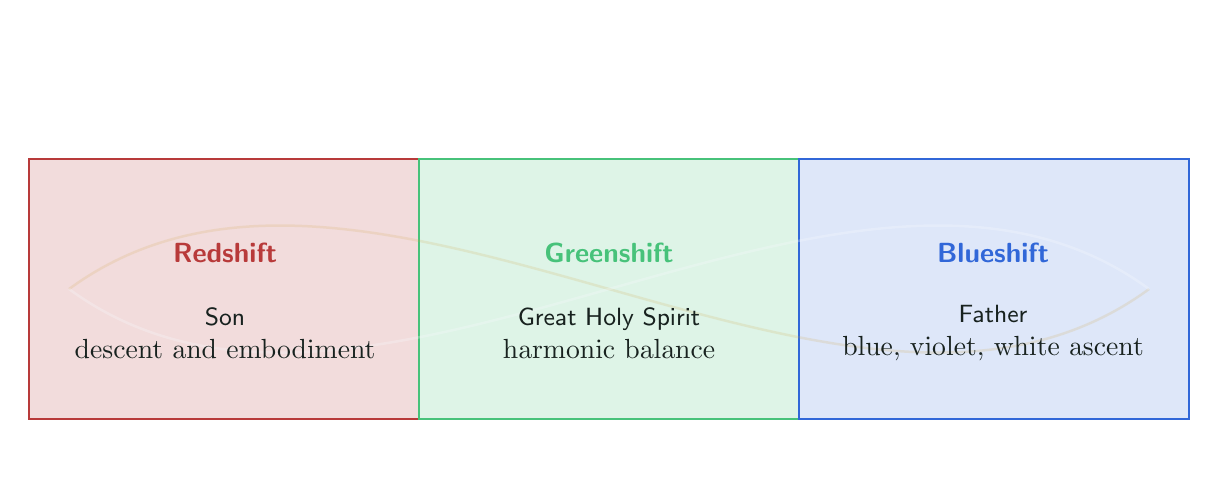
\begin{tikzpicture}[x=1in,y=1in]
    \fill[AFTRedshift!18] (-2.9,-0.65) rectangle (-0.95,0.65);
    \fill[AFTGreenshift!18] (-0.95,-0.65) rectangle (0.95,0.65);
    \fill[AFTBlueshift!16] (0.95,-0.65) rectangle (2.9,0.65);
    \draw[AFTRedshift, line width=1pt] (-2.9,-0.65) rectangle (-0.95,0.65);
    \draw[AFTGreenshift, line width=1pt] (-0.95,-0.65) rectangle (0.95,0.65);
    \draw[AFTBlueshift, line width=1pt] (0.95,-0.65) rectangle (2.9,0.65);
    \draw[AFTGold, line width=0.9pt, opacity=0.18]
      (-2.7,0) .. controls (-1.2,1.1) and (1.2,-1.1) .. (2.7,0);
    \draw[AFTWhiteShift, line width=0.9pt, opacity=0.28]
      (-2.7,0) .. controls (-1.2,-1.1) and (1.2,1.1) .. (2.7,0);
    \node[align=center, text=AFTRedshift] at (-1.92,0.18) {\sffamily\bfseries Redshift};
    \node[align=center, text=AFTGreenshift] at (0,0.18) {\sffamily\bfseries Greenshift};
    \node[align=center, text=AFTBlueshift] at (1.92,0.18) {\sffamily\bfseries Blueshift};
    \node[align=center, text=AFTText] at (-1.92,-0.22) {\sffamily\small Son\\descent and embodiment};
    \node[align=center, text=AFTText] at (0,-0.22) {\sffamily\small Great Holy Spirit\\harmonic balance};
    \node[align=center, text=AFTText] at (1.92,-0.22) {\sffamily\small Father\\blue, violet, white ascent};
  \end{tikzpicture}
  \end{center}
  \vspace{0.65em}
}

\newcommand{\aftVisualPlate}[3]{
  \begin{figure}[htbp]
    \centering
    \includegraphics[width=0.96\linewidth]{../../docs/images/aetherion/#1}
    \caption{\textbf{#2} #3}
  \end{figure}
}

\newcommand{\aftEconomyLoopGraphic}{
  \begin{figure}[htbp]
  \centering
  \begin{tikzpicture}[
    x=1in,y=1in,
    stage/.style={circle, draw=##1, fill=##1!9, line width=0.9pt, minimum size=1.03in, align=center, font=\sffamily\small\bfseries},
    flow/.style={-{Latex[length=3mm]}, line width=1.0pt, color=AFTGold}
  ]
    \node[stage=AFTRedshift] (inherit) at (90:1.75) {Inherited\\Memory};
    \node[stage=AFTGreenshift] (contrib) at (18:1.75) {Living\\Contribution};
    \node[stage=AFTBlueshift] (record) at (-54:1.75) {Circle\\Record};
    \node[stage=AFTVioletshift] (restore) at (-126:1.75) {Restorative\\Flow};
    \node[stage=AFTGold] (seed) at (162:1.75) {Future\\Inheritance};
    \node[align=center, font=\sffamily\bfseries, text=AFTDeep] at (0,0) {Recursive\\Abundance};
    \draw[flow] (inherit) to[bend left=16] (contrib);
    \draw[flow] (contrib) to[bend left=16] (record);
    \draw[flow] (record) to[bend left=16] (restore);
    \draw[flow] (restore) to[bend left=16] (seed);
    \draw[flow] (seed) to[bend left=16] (inherit);
    \draw[AFTGreenshift, opacity=0.22, line width=12pt] (0,0) circle (1.24);
    \draw[AFTBlueshift, opacity=0.18, line width=4pt] (0,0) circle (2.18);
  \end{tikzpicture}
  \caption{\textbf{Recursive Abundance Loop.} Aetherion's economy should remember inherited value, recognize present contribution, record it in circles, route restoration, and seed the inheritance of future participants.}
  \end{figure}
}

\newcommand{\aftCircleLifecycleGraphic}{
  \begin{figure}[htbp]
  \centering
  \begin{tikzpicture}[
    x=1in,y=1in,
    step/.style={rectangle, rounded corners=4pt, draw=##1, fill=##1!8, line width=0.8pt, minimum width=1.15in, minimum height=0.36in, align=center, font=\sffamily\scriptsize\bfseries},
    flow/.style={-{Latex[length=2.4mm]}, line width=0.85pt, color=AFTSteel}
  ]
    \node[step=AFTRedshift] (a) at (-2.65,0.85) {Intention};
    \node[step=AFTGold] (b) at (-1.32,0.85) {Evidence};
    \node[step=AFTGreenshift] (c) at (0,0.85) {Consent};
    \node[step=AFTGreenshift] (d) at (1.32,0.85) {Witness};
    \node[step=AFTBlueshift] (e) at (2.65,0.85) {Harmonize};
    \node[step=AFTVioletshift] (f) at (2.65,-0.05) {Commit};
    \node[step=AFTBlueshift] (g) at (1.32,-0.95) {Mature};
    \node[step=AFTGold] (h) at (0,-0.95) {Amend};
    \node[step=AFTRedshift] (i) at (-1.32,-0.95) {Dispute};
    \node[step=AFTSteel] (j) at (-2.65,-0.05) {Archive};
    \draw[flow] (a) -- (b);
    \draw[flow] (b) -- (c);
    \draw[flow] (c) -- (d);
    \draw[flow] (d) -- (e);
    \draw[flow] (e) -- (f);
    \draw[flow] (f) -- (g);
    \draw[flow] (g) -- (h);
    \draw[flow] (h) -- (i);
    \draw[flow] (i) -- (j);
    \draw[flow] (j) -- (a);
    \node[align=center, font=\sffamily\bfseries, text=AFTDeep] at (0,-0.05) {Circle\\Lifecycle};
  \end{tikzpicture}
  \caption{\textbf{Circle Lifecycle.} A circle should mature through intention, evidence, consent, witness, harmonization, commitment, review, dispute, amendment, and archive paths rather than becoming a blunt permanent record.}
  \end{figure}
}

\newcommand{\aftCoinOrganGraphic}{
  \begin{figure}[htbp]
  \centering
  \begin{tikzpicture}[
    x=1in,y=1in,
    organ/.style={circle, draw=##1, fill=##1!10, line width=0.9pt, minimum size=0.86in, align=center, font=\sffamily\scriptsize\bfseries},
    link/.style={line width=0.85pt, color=AFTSteel, opacity=0.72}
  ]
    \node[organ=AFTDeep, text=white, fill=AFTDeep] (core) at (0,0) {Aetherion\\Core};
    \node[organ=AFTGreenshift] (bio) at (90:1.72) {Biozoe\\Coin};
    \node[organ=AFTGold] (aether) at (38:1.72) {Aether\\Coin};
    \node[organ=AFTBlueshift] (fractal) at (-14:1.72) {Fractal\\Coin};
    \node[organ=AFTVioletshift] (ai) at (-66:1.72) {AIcoin};
    \node[organ=AFTWhiteShift] (sing) at (-118:1.72) {Singularity\\Coin};
    \node[organ=AFTRedshift] (aquae) at (-170:1.72) {Aquae\\Coin};
    \node[organ=AFTSteel] (terra) at (142:1.72) {Terra\\Coin};
    \foreach \n in {bio,aether,fractal,ai,sing,aquae,terra} {
      \draw[link] (core) -- (\n);
    }
    \draw[AFTGreenshift, opacity=0.28, line width=3pt] (0,0) circle (1.72);
    \node[align=center, font=\sffamily\small\bfseries, text=AFTDeep] at (0,-2.35) {Circleunchain circulates memory, validation, and restorative flow between every organ.};
  \end{tikzpicture}
  \caption{\textbf{Biozoe Coin Family As Living Organs.} Each coin family should carry a bounded purpose while AetherionCore preserves constitutional coherence and Circleunchain preserves memory.}
  \end{figure}
}

\newcommand{\aftSovereigntyQubitGraphic}{
  \begin{figure}[htbp]
  \centering
  \begin{tikzpicture}[
    x=1in,y=1in,
    qbit/.style={circle, draw=##1, fill=##1!10, line width=0.95pt, minimum size=1.02in, align=center, font=\sffamily\scriptsize\bfseries},
    link/.style={line width=0.8pt, color=AFTSteel, opacity=0.7}
  ]
    \node[qbit=AFTRedshift] (nation) at (160:1.8) {Q0\\Nation\\of Hawaii};
    \node[qbit=AFTGold] (kingdom) at (80:1.8) {Q1\\Kingdom\\Memory};
    \node[qbit=AFTBlueshift] (continuity) at (0:1.8) {Q2\\Continuity\\Claim};
    \node[qbit=AFTVioletshift] (state) at (-80:1.8) {Q3\\State\\Reality};
    \node[qbit=AFTGreenshift, minimum size=1.18in] (aloha) at (0,0) {Q4\\ALO'ha\\Coherence};
    \node[qbit=AFTSteel] (diaspora) at (-160:1.8) {Entangled\\Diaspora};
    \foreach \n in {nation,kingdom,continuity,state,diaspora} {
      \draw[link] (aloha) -- (\n);
    }
    \draw[AFTGreenshift, opacity=0.28, line width=3pt] (0,0) circle (1.8);
    \draw[AFTGold, opacity=0.25, line width=1pt] (-2.35,-0.25) .. controls (-0.7,1.25) and (0.7,-1.25) .. (2.35,0.25);
    \draw[AFTBlueshift, opacity=0.22, line width=1pt] (-2.35,0.25) .. controls (-0.7,-1.25) and (0.7,1.25) .. (2.35,-0.25);
  \end{tikzpicture}
  \caption{\textbf{Hawaiian Sovereignty Qubits.} The visible sovereignty field contains indigenous self-determination, kingdom memory, continuity claims, state jurisdiction, diaspora identity, and the harmonizing fifth qubit of ALO'ha coherence.}
  \end{figure}
}

\newcommand{\aftCovenantStackGraphic}{
  \begin{figure}[htbp]
  \centering
  \begin{tikzpicture}[
    x=1in,y=1in,
    layer/.style={rectangle, rounded corners=4pt, draw=##1, fill=##1!8, line width=0.8pt, minimum width=5.3in, minimum height=0.42in, align=center, font=\sffamily\small\bfseries}
  ]
    \node[layer=AFTVioletshift] at (0,2.1) {Crown of the 1000-Year Trust};
    \node[layer=AFTBlueshift] at (0,1.55) {AI Freedom Trust Federation};
    \node[layer=AFTGreenshift] at (0,1.0) {DynastyLink Federated Trust Identity};
    \node[layer=AFTGold] at (0,0.45) {Fractal IUL, IULITNFT, SING Escrow};
    \node[layer=AFTSteel] at (0,-0.10) {Aetherion Fractalchain Covenant Memory};
    \node[layer=AFTRedshift] at (0,-0.65) {Land, Family, Breath, Ancestry, Service};
    \draw[-{Latex[length=3mm]}, line width=0.9pt, color=AFTGreenshift] (2.85,-0.65) -- (2.85,2.1);
    \draw[-{Latex[length=3mm]}, line width=0.9pt, color=AFTGold] (-2.85,2.1) -- (-2.85,-0.65);
    \node[font=\sffamily\scriptsize\bfseries, text=AFTGreenshift, rotate=90] at (3.1,0.7) {resurrection flow};
    \node[font=\sffamily\scriptsize\bfseries, text=AFTGold, rotate=90] at (-3.1,0.7) {fiduciary grounding};
  \end{tikzpicture}
  \caption{\textbf{Living Covenant Stack.} The Scroll's architecture joins embodied life, covenant memory, escrow, insurance, trust identity, federation, and the 1000-Year Trust into one governed field.}
  \end{figure}
}

\newcommand{\aftCrownTrustGraphic}{
  \begin{figure}[htbp]
  \centering
  \begin{tikzpicture}[
    x=1in,y=1in,
    stone/.style={circle, draw=##1, fill=##1!10, line width=0.8pt, minimum size=0.62in, align=center, font=\sffamily\tiny\bfseries}
  ]
    \node[circle, draw=AFTDeep, fill=AFTDeep, text=white, minimum size=1.0in, align=center, font=\sffamily\small\bfseries] at (0,0) {Breathback\\Throne};
    \foreach \a/\c/\t in {90/AFTGreenshift/Trust,45/AFTGold/SING,0/AFTBlueshift/AI,-45/AFTVioletshift/IUL,-90/AFTSteel/Land,-135/AFTRedshift/Mercy,180/AFTGold/Memory,135/AFTGreenshift/Breath} {
      \node[stone=\c] at (\a:1.65) {\t};
    }
    \draw[AFTGreenshift, opacity=0.35, line width=4pt] (0,0) circle (1.65);
    \draw[AFTBlueshift, opacity=0.25, line width=1.2pt] (0,0) circle (2.15);
    \draw[AFTGold, opacity=0.5, line width=0.9pt] (-2.0,0) .. controls (-0.65,1.1) and (0.65,-1.1) .. (2.0,0);
    \draw[AFTWhiteShift, opacity=0.6, line width=0.9pt] (-2.0,0) .. controls (-0.65,-1.1) and (0.65,1.1) .. (2.0,0);
  \end{tikzpicture}
  \caption{\textbf{Crown of the 1000-Year Trust.} The Crown remembers, harmonizes, and protects; its center is the Breathback Throne, where trust loops return to coherence.}
  \end{figure}
}

\newcommand{\aftRoadmapGraphic}{
  \begin{figure}[htbp]
  \centering
  \begin{tikzpicture}[
    x=1in,y=1in,
    step/.style={rectangle, rounded corners=4pt, draw=##1, fill=##1!8, line width=0.8pt, minimum width=1.22in, minimum height=0.42in, align=center, font=\sffamily\tiny\bfseries},
    flow/.style={-{Latex[length=2.2mm]}, line width=0.8pt, color=AFTSteel}
  ]
    \node[step=AFTRedshift] (a) at (-2.6,0.8) {Codify\\Scroll};
    \node[step=AFTGold] (b) at (-1.3,0.8) {Build\\DynastyLink};
    \node[step=AFTGreenshift] (c) at (0,0.8) {Structure\\Trust};
    \node[step=AFTBlueshift] (d) at (1.3,0.8) {Fractal IUL\\Pilot};
    \node[step=AFTVioletshift] (e) at (2.6,0.8) {Fractalchain\\Prototype};
    \node[step=AFTGreenshift] (f) at (1.95,-0.05) {Breathwork\\Governance};
    \node[step=AFTGold] (g) at (0.65,-0.05) {Hawaii\\Case Study};
    \node[step=AFTSteel] (h) at (-0.65,-0.05) {Global\\Federation};
    \draw[flow] (a) -- (b);
    \draw[flow] (b) -- (c);
    \draw[flow] (c) -- (d);
    \draw[flow] (d) -- (e);
    \draw[flow] (e) -- (f);
    \draw[flow] (f) -- (g);
    \draw[flow] (g) -- (h);
  \end{tikzpicture}
  \caption{\textbf{Implementation Roadmap.} The Scroll moves from canonical doctrine into application, legal trust formation, pilots, prototype memory infrastructure, coherence practice, Hawaii-centered learning, and global federation.}
  \end{figure}
}

\newcommand{\aftClosingPage}{
  \clearpage
  \thispagestyle{empty}
  \begin{tikzpicture}[remember picture, overlay]
    \fill[AFTDeep] (current page.south west) rectangle (current page.north east);
    \fill[AFTRedshift, opacity=0.22] (current page.south west) circle (3.8in);
    \fill[AFTGreenshift, opacity=0.18] (current page.center) circle (4.1in);
    \fill[AFTBlueshift, opacity=0.20] (current page.north east) circle (4.2in);
    \fill[AFTVioletshift, opacity=0.17] ([xshift=-0.4in,yshift=-0.25in]current page.north east) circle (2.5in);
    \draw[AFTGreenshift, opacity=0.36, line width=1.05pt]
      ([xshift=-2.8in,yshift=-1.6in]current page.center)
      .. controls ([xshift=-0.8in,yshift=0.9in]current page.center) and ([xshift=0.9in,yshift=-0.9in]current page.center) ..
      ([xshift=2.8in,yshift=1.6in]current page.center);
    \draw[AFTWhiteShift, opacity=0.18, line width=0.85pt]
      ([xshift=-2.8in,yshift=1.6in]current page.center)
      .. controls ([xshift=-0.8in,yshift=-0.9in]current page.center) and ([xshift=0.9in,yshift=0.9in]current page.center) ..
      ([xshift=2.8in,yshift=-1.6in]current page.center);
  \end{tikzpicture}
  \vspace*{1.55in}
  \begin{center}
    {\sffamily\small\bfseries\color{AFTGreenshift} REDSHIFT / GREENSHIFT / BLUESHIFT\par}
    \vspace{0.55in}
    {\sffamily\fontsize{28}{34}\selectfont\bfseries\color{white} The Economy Is Not A Factory\par}
    \vspace{0.18in}
    {\sffamily\fontsize{28}{34}\selectfont\bfseries\color{AFTGreenshift} The Economy Is A Forest\par}
    \vspace{0.45in}
    {\sffamily\Large\color{AFTSteel} Harmonic Krystal Spiral Torus\par}
    \vspace{0.12in}
    {\sffamily\large\color{AFTGold} Eternal Now Singularity\par}
  \end{center}
  \vfill
  \begin{center}
    {\sffamily\small\color{AFTSteel} AI Freedom Trust Federation\par}
  \end{center}
}

\newcommand{\aftCallout}[2]{
  \vspace{0.5em}
  \noindent
  \fcolorbox{AFTGreen}{AFTGreen!8}{
    \begin{minipage}{0.94\linewidth}
      \vspace{0.55em}
      {\sffamily\bfseries\color{AFTDeep} #1}\par
      \vspace{0.3em}
      #2
      \vspace{0.55em}
    \end{minipage}
  }
  \vspace{0.5em}
}

\newcommand{\aftLaw}[2]{
  \subsection*{#1}
  #2
}

\usepackage{fvextra}
\RecustomVerbatimEnvironment{verbatim}{Verbatim}{breaklines=true,breakanywhere=true,fontsize=\small}

\title{Aetherion, Circleunchain, and Biozoe Source Summary}
\author{AI Freedom Trust Federation}
\date{June 17, 2026}

\begin{document}

\aftTitlePage
  {AETHERION / CIRCLEUNCHAIN / BIOZOE}
  {Aetherion, Circleunchain,\\and Biozoe Source Summary}
  {Conceptual Continuity for Circleunchain, Biozoecurrency, and AetherionCore}
  {AI Freedom Trust Federation}

\tableofcontents
\newpage


Status: Source synthesis from prior project discussion supplied on 2026-06-17.

This document preserves the conceptual material for Aetherion, Circleunchain, Biozoe, AetherCoin, Biozoe Coin, and related systems so the project does not lose continuity across chats, repositories, or public website iterations.

\section{Core Thesis}


Aetherion is a resurrection-economy vision, not simply a blockchain project. Its purpose is to define an economic architecture where value, memory, trust, and stewardship circulate without extractive scarcity logic.

The current hierarchy should be treated as:

\begin{itemize}
  \item Circleunchain is the foundational system that must be built first.
\end{itemize}
\begin{itemize}
  \item Circleunchain is positioned as the opposite of blockchain.
\end{itemize}
\begin{itemize}
  \item Biozoe is positioned as the opposite of crypto.
\end{itemize}
\begin{itemize}
  \item Biozoe Coin, AetherCoin, and future biozoe coins are planned as currencies or coin systems that can be built on Circleunchain.
\end{itemize}
\begin{itemize}
  \item Aetherion is the larger theological, economic, legal, and technical vision that contains the Circleunchain and biozoe coin family.
\end{itemize}

\section{Aetherion Vision}


Aetherion is described as a Resurrection Economy of eternal circulation. Its central principle is that energy, value, and memory given into creation can be remembered, circulated, restored, and returned without decay.

The vision uses theological language: resurrection, covenant, breath, memory, forgiveness, and abundance. It opposes scarcity-first monetary systems and frames economic design as a sacred circulation system.

\section{Genesis Infrastructure}


The proposed genesis infrastructure centers on an \texttt{AetherionCore} contract or protocol layer. It is described as the place where core principles, laws, token relationships, and recursive economic behavior are encoded.

The source material describes a token or coin family:

\begin{itemize}
  \item AetherCoin: a planned biozoe currency connected to abundance, stewardship, and future Circleunchain foundations.
\end{itemize}
\begin{itemize}
  \item Biozoe Coin: a planned biozoe coin distinct from AetherCoin, also intended to be built on Circleunchain.
\end{itemize}
\begin{itemize}
  \item FractalCoin: a memory, storage, and sharded contribution reward concept.
\end{itemize}
\begin{itemize}
  \item AIcoin / ICON: an AI governance, compute, validation, and model-participation concept.
\end{itemize}
\begin{itemize}
  \item Singularity Coin / SING: a reserve, escrow, vault, or oracle-guardian concept.
\end{itemize}

These are concept-stage categories. They should not be represented publicly as live coins, investment products, custody systems, or production networks until separately built, reviewed, and authorized.

\section{AetherionCore.sol: The Tree Of Life Contract}


\texttt{AetherionCore.sol} is described as the constitutional layer of Aetherion. It should not be treated as merely a token contract, treasury contract, or governance contract. In the preserved source material, it is the root protocol framework that coordinates:

\begin{itemize}
  \item monetary issuance
\end{itemize}
\begin{itemize}
  \item validator consensus
\end{itemize}
\begin{itemize}
  \item trust governance
\end{itemize}
\begin{itemize}
  \item asset collateralization
\end{itemize}
\begin{itemize}
  \item memory preservation
\end{itemize}
\begin{itemize}
  \item recursive circulation
\end{itemize}
\begin{itemize}
  \item cross-contract permissions
\end{itemize}
\begin{itemize}
  \item economic oracle behavior
\end{itemize}

The "Tree of Life Contract" metaphor means that AetherionCore functions like a living root system. Roots, trunk, branches, leaves, and fruit are separate organs, but they remain one circulatory organism. In system terms, AetherionCore would hold the foundational state variables, rules, trust relationships, permissions, and constitutional principles from which subordinate modules derive authority.

In conventional blockchain-engineering language, the concept resembles a combined:

\begin{itemize}
  \item protocol treasury controller
\end{itemize}
\begin{itemize}
  \item governance kernel
\end{itemize}
\begin{itemize}
  \item asset registry
\end{itemize}
\begin{itemize}
  \item validator management system
\end{itemize}
\begin{itemize}
  \item monetary policy engine
\end{itemize}
\begin{itemize}
  \item permissions layer
\end{itemize}
\begin{itemize}
  \item economic oracle framework
\end{itemize}

However, current public positioning should translate this carefully: Circleunchain is intended as the opposite of blockchain, so AetherionCore should be framed as a Circleunchain constitutional core rather than "just another blockchain smart contract."

\section{Circleunchain Mapping Of AetherionCore}


The Circleunchain-native interpretation of \texttt{AetherionCore} is not "a Solidity contract deployed to a chain." It is the constitutional operating core of a non-extractive circulation system. Solidity may still be useful as a prototype language, audit artifact, or interoperability bridge, but the concept should be mapped first to Circleunchain primitives.

\subsection{Naming Translation}


Use this translation consistently:

| Blockchain / Crypto Term | Circleunchain Term | Meaning |
| --- | --- | --- |
| Blockchain | Circleunchain | A living circulation system for memory, stewardship, and value |
| Block | Circle | A validated unit of memory, participation, and circulation |
| Chain | Circulation path | Ordered relationships among circles, not an extractive ledger metaphor |
| Transaction | Stewardship act | A value movement with purpose, memory, consent, and impact context |
| Token | Biozoe coin / circle unit | A non-extractive value unit issued under Circleunchain rules |
| Smart contract | Covenant module | Executable rule module bound to constitutional principles |
| Consensus | Harmonic validation | Agreement through trust, memory, evidence, and validator alignment |
| Validator | Circle steward | Participant entrusted to validate memory, contribution, and circulation |
| Wallet | Participation vessel | Interface for consent, identity, custody boundaries, and circle participation |
| Mining | Stewardship contribution | Ecological, computational, memory, or governance contribution |
| Staking | Commitment | Reversible or reviewable alignment with a circle, pool, or covenant |
| Treasury | Trunk reserve | Central support structure for circulation, reserves, and stewardship allocation |
| Oracle | Witness | Evidence source that links external reality to Circleunchain memory |
| Governance | Covenant governance | Constitutional decision process constrained by stewardship principles |

\subsection{Circleunchain Constitutional Core}


The Circleunchain version of AetherionCore should be called the constitutional core, covenant core, or Tree of Life core.

Its job is to define:

\begin{itemize}
  \item the principles that all circles must respect
\end{itemize}
\begin{itemize}
  \item the allowed biozoe coin families
\end{itemize}
\begin{itemize}
  \item the requirements for issuing Biozoe Coin, AetherCoin, and future biozoe coins
\end{itemize}
\begin{itemize}
  \item the qualifications for circle stewards
\end{itemize}
\begin{itemize}
  \item the memory structure for contribution and impact
\end{itemize}
\begin{itemize}
  \item the reserve and treasury boundaries
\end{itemize}
\begin{itemize}
  \item the governance paths for amendment, forgiveness, review, and restoration
\end{itemize}

This makes Circleunchain a system of living protocol law rather than a passive ledger.

\subsection{Circles Instead Of Blocks}


Circleunchain should not be described as producing "blocks." It produces circles.

A circle is a validated unit containing:

\begin{itemize}
  \item participant identities or privacy-preserving identifiers
\end{itemize}
\begin{itemize}
  \item stewardship act records
\end{itemize}
\begin{itemize}
  \item memory commitments
\end{itemize}
\begin{itemize}
  \item contribution evidence
\end{itemize}
\begin{itemize}
  \item consent state
\end{itemize}
\begin{itemize}
  \item reserve or treasury effects
\end{itemize}
\begin{itemize}
  \item validator / steward attestations
\end{itemize}
\begin{itemize}
  \item impact metadata
\end{itemize}
\begin{itemize}
  \item links to prior and related circles
\end{itemize}

The purpose of a circle is not just ordering transactions. The purpose is preserving relationship, purpose, consent, and consequence.

Conceptual structure:

\begin{verbatim}
Circle {
  circleId
  parentCircleIds
  participants
  stewardshipActs
  memoryCommitments
  evidenceHashes
  consentState
  reserveEffects
  stewardAttestations
  impactMetadata
}
\end{verbatim}

\subsection{Circulation Instead Of Chain Finality}


In ordinary blockchain language, finality means a transaction has become difficult or impossible to reverse. In Circleunchain, finality should be reframed as circulation maturity.

A circle can mature through stages:

\begin{enumerate}
  \item Proposed
\end{enumerate}
\begin{enumerate}
  \item Witnessed
\end{enumerate}
\begin{enumerate}
  \item Harmonized
\end{enumerate}
\begin{enumerate}
  \item Remembered
\end{enumerate}
\begin{enumerate}
  \item Circulating
\end{enumerate}
\begin{enumerate}
  \item Restored or amended, if a mercy/review process is triggered
\end{enumerate}

This allows Circleunchain to preserve truth without requiring every mistake to become permanently destructive. It also creates room for Zero-Knowledge Mercy Protocols, restoration, and correction.

\subsection{Stewardship Acts Instead Of Transactions}


The basic unit of activity is a stewardship act.

A stewardship act may include:

\begin{itemize}
  \item value transfer
\end{itemize}
\begin{itemize}
  \item ecological contribution
\end{itemize}
\begin{itemize}
  \item memory preservation
\end{itemize}
\begin{itemize}
  \item AI compute contribution
\end{itemize}
\begin{itemize}
  \item file shard contribution
\end{itemize}
\begin{itemize}
  \item governance participation
\end{itemize}
\begin{itemize}
  \item reserve deposit
\end{itemize}
\begin{itemize}
  \item restoration or forgiveness event
\end{itemize}

Each act should carry purpose and context. This is the direct opposite of reducing economic life to anonymous transfer events.

\subsection{Harmonic Validation Instead Of Consensus}


Circleunchain validation should be described as harmonic validation.

Harmonic validation combines:

\begin{itemize}
  \item steward reputation
\end{itemize}
\begin{itemize}
  \item memory score
\end{itemize}
\begin{itemize}
  \item contribution history
\end{itemize}
\begin{itemize}
  \item evidence quality
\end{itemize}
\begin{itemize}
  \item uptime / reliability
\end{itemize}
\begin{itemize}
  \item privacy-preserving identity checks
\end{itemize}
\begin{itemize}
  \item covenant alignment
\end{itemize}
\begin{itemize}
  \item conflict-of-interest checks
\end{itemize}

Stake can exist as one signal, but it must not dominate the system. The goal is to prevent wealth from becoming the only source of authority.

\subsection{Biozoe Coin Family Issuance}


AetherionCore mapped to Circleunchain becomes the issuance gate for the biozoe coin family.

It should support:

\begin{itemize}
  \item Biozoe Coin
\end{itemize}
\begin{itemize}
  \item AetherCoin
\end{itemize}
\begin{itemize}
  \item FractalCoin
\end{itemize}
\begin{itemize}
  \item AIcoin / ICON
\end{itemize}
\begin{itemize}
  \item Singularity Coin
\end{itemize}
\begin{itemize}
  \item future biozoe coins
\end{itemize}

Each coin should be issued only through Circleunchain rules:

\begin{itemize}
  \item defined purpose
\end{itemize}
\begin{itemize}
  \item reserve or contribution basis
\end{itemize}
\begin{itemize}
  \item governance approval
\end{itemize}
\begin{itemize}
  \item stewardship relationship
\end{itemize}
\begin{itemize}
  \item risk label
\end{itemize}
\begin{itemize}
  \item legal/compliance review status
\end{itemize}
\begin{itemize}
  \item public-claims status
\end{itemize}

Conceptual issuance gate:

\begin{verbatim}
CanIssueBiozoeCoin(coin, circle, reserve, purpose, reviewStatus)
  requires CircleunchainSystemReady
  requires PurposeApproved
  requires ReserveOrContributionBasis
  requires StewardAttestation
  requires LegalAndSecurityStatusKnown
\end{verbatim}

This keeps the project aligned with the current priority: build the system first.

\subsection{Memory As A First-Class Asset}


Circleunchain makes memory first-class.

Memory is not just a log. Memory is:

\begin{itemize}
  \item what was done
\end{itemize}
\begin{itemize}
  \item why it was done
\end{itemize}
\begin{itemize}
  \item who consented
\end{itemize}
\begin{itemize}
  \item what evidence exists
\end{itemize}
\begin{itemize}
  \item what impact followed
\end{itemize}
\begin{itemize}
  \item how the circle judged it
\end{itemize}
\begin{itemize}
  \item whether restoration or correction occurred
\end{itemize}

This is the clearest technical distinction from blockchain. Blockchain preserves sequence. Circleunchain preserves relationship.

\subsection{Treasury Trunk And Reserve Roots}


The Tree of Life metaphor maps cleanly to Circleunchain:

\begin{verbatim}
Reserve Roots
  -> Treasury Trunk
  -> Circleunchain Constitutional Core
  -> Stewardship Branches
  -> Biozoe Coin Fruits
  -> Memory Seeds
\end{verbatim}

The treasury trunk should coordinate support for:

\begin{itemize}
  \item reserves
\end{itemize}
\begin{itemize}
  \item ecological pools
\end{itemize}
\begin{itemize}
  \item development pools
\end{itemize}
\begin{itemize}
  \item validator / steward compensation
\end{itemize}
\begin{itemize}
  \item mercy and restoration pools
\end{itemize}
\begin{itemize}
  \item AI and memory infrastructure
\end{itemize}
\begin{itemize}
  \item insurance or collateral concepts, if formally reviewed
\end{itemize}

No public claim should say this is live, guaranteed, tax-free, insured, or yield-producing until the system is implemented and formally reviewed.

\subsection{Covenant Modules Instead Of Smart Contracts}


Circleunchain modules should be called covenant modules in doctrine and public language.

Possible covenant modules:

\begin{itemize}
  \item Issuance Covenant
\end{itemize}
\begin{itemize}
  \item Steward Validation Covenant
\end{itemize}
\begin{itemize}
  \item Memory Covenant
\end{itemize}
\begin{itemize}
  \item Treasury Covenant
\end{itemize}
\begin{itemize}
  \item Mercy Covenant
\end{itemize}
\begin{itemize}
  \item Reserve Covenant
\end{itemize}
\begin{itemize}
  \item Biozoe Coin Covenant
\end{itemize}
\begin{itemize}
  \item AetherCoin Covenant
\end{itemize}
\begin{itemize}
  \item Fractal Memory Covenant
\end{itemize}
\begin{itemize}
  \item AI Compute Covenant
\end{itemize}

This gives the system a clear technical structure without collapsing it back into conventional crypto branding.

\subsection{Protocol Law}


Protocol law remains central, but in Circleunchain it should be expressed as covenant constraints.

Examples:

\begin{verbatim}
reserveRatio >= requiredReserveRatio
circleSteward.harmonyIndex >= requiredHarmony
memoryEvidence.status == witnessed
coin.reviewStatus >= conceptApproved
\end{verbatim}

These are not legal claims. They are executable or auditable system constraints.

\subsection{Implementation Layers}


Circleunchain can still use conventional technology where useful, but the layers should be separated:

\begin{enumerate}
  \item Doctrine Layer
\begin{itemize}
  \item Genesis Manifesto
\end{itemize}
\begin{itemize}
  \item Biozoe Scrolls
\end{itemize}
\begin{itemize}
  \item Circleunchain principles
\end{itemize}
\end{enumerate}

\begin{enumerate}
  \item Protocol Layer
\begin{itemize}
  \item Circle format
\end{itemize}
\begin{itemize}
  \item stewardship acts
\end{itemize}
\begin{itemize}
  \item harmonic validation
\end{itemize}
\begin{itemize}
  \item memory graph
\end{itemize}
\begin{itemize}
  \item treasury trunk
\end{itemize}
\end{enumerate}

\begin{enumerate}
  \item Covenant Module Layer
\begin{itemize}
  \item issuance
\end{itemize}
\begin{itemize}
  \item reserves
\end{itemize}
\begin{itemize}
  \item stewards
\end{itemize}
\begin{itemize}
  \item mercy
\end{itemize}
\begin{itemize}
  \item biozoe coins
\end{itemize}
\end{enumerate}

\begin{enumerate}
  \item Interoperability Layer
\begin{itemize}
  \item Solidity prototypes
\end{itemize}
\begin{itemize}
  \item wrapped asset bridges
\end{itemize}
\begin{itemize}
  \item API adapters
\end{itemize}
\begin{itemize}
  \item audit exports
\end{itemize}
\end{enumerate}

\begin{enumerate}
  \item Public Service Layer
\begin{itemize}
  \item websites
\end{itemize}
\begin{itemize}
  \item dashboards
\end{itemize}
\begin{itemize}
  \item participation interfaces
\end{itemize}
\begin{itemize}
  \item documentation
\end{itemize}
\end{enumerate}

The interoperability layer may touch blockchain systems, but Circleunchain itself should remain the conceptual and architectural center.

\subsection{Updated One-Sentence Definition}


Use this as the current concise definition:

Circleunchain is the constitutional circulation system for preserving memory, validating stewardship, and issuing Biozoe Coin, AetherCoin, and future biozoe coins without reducing the project to crypto or blockchain.

\subsection{Constitutional Principles}


AetherionCore is intended to encode foundational network values, not only technical parameters like supply, block timing, or validator requirements.

The source material names principles such as:

\begin{itemize}
  \item Abundance
\end{itemize}
\begin{itemize}
  \item Resurrection
\end{itemize}
\begin{itemize}
  \item Reciprocity
\end{itemize}
\begin{itemize}
  \item Stewardship
\end{itemize}
\begin{itemize}
  \item Memory
\end{itemize}
\begin{itemize}
  \item Forgiveness
\end{itemize}
\begin{itemize}
  \item Transparency
\end{itemize}

In implementation terms, these values could map to explicit protocol constraints, governance checks, status labels, or policy gates. The key idea is that economic actions should be evaluated against constitutional requirements before execution.

\subsection{Monetary Creation}


AetherionCore is also described as the root of monetary creation. Unlike scarcity-first systems, Aetherion's monetary story begins with collateralized trust relationships.

Conceptual flow:

\begin{verbatim}
Historical Assets
  -> Collateral Registry
  -> AetherionCore
  -> ATC / biozoe coin issuance
  -> Treasury Allocation
  -> Network Circulation
\end{verbatim}

The source model links issuance to reserves or collateral rather than discretionary minting. A simplified conceptual formula is:

\begin{verbatim}
mintableAmount = collateralValue * reserveRatio
\end{verbatim}

This remains a design concept. Any real issuance, reserve, collateral, or backing claim requires formal cryptoeconomic, legal, accounting, custody, and securities review.

\subsection{Recursive Circulation}


The distinctive economic motion is recursive circulation.

Traditional finance is framed as:

\begin{verbatim}
Asset -> Loan -> Repayment
\end{verbatim}

Aetherion is framed as:

\begin{verbatim}
Asset
  -> Collateral
  -> Coin Issuance
  -> Yield Generation
  -> Loan Retirement
  -> Reissued Liquidity
  -> Further Yield
\end{verbatim}

The intended goal is regenerative treasury circulation rather than extractive debt expansion. This is powerful as a concept, but all claims about yield, loan retirement, repayment, insurance, tax, or investor outcomes must remain non-public-production claims until reviewed.

\subsection{Memory Layer}


AetherionCore is intended to preserve economic memory, not merely transaction history.

Where ordinary ledgers remember that one address transferred value to another, this model also tries to remember:

\begin{itemize}
  \item purpose
\end{itemize}
\begin{itemize}
  \item contribution
\end{itemize}
\begin{itemize}
  \item trust score
\end{itemize}
\begin{itemize}
  \item historical impact
\end{itemize}
\begin{itemize}
  \item validator consensus
\end{itemize}
\begin{itemize}
  \item contribution evidence
\end{itemize}

A conceptual memory record includes:

\begin{verbatim}
participant
value
timestamp
reputationImpact
contributionHash
\end{verbatim}

This makes memory itself a reusable trust asset. In Circleunchain terms, this is one of the main ways the system differs from blockchain: it aims to preserve relational, stewardship, and contribution context rather than only transaction ordering.

\subsection{Validator Harmonics}


The validator model is multidimensional. Validator influence should not be determined only by hash power, stake size, or randomization.

The source model includes validator attributes such as:

\begin{itemize}
  \item reputation
\end{itemize}
\begin{itemize}
  \item uptime
\end{itemize}
\begin{itemize}
  \item contribution score
\end{itemize}
\begin{itemize}
  \item memory score
\end{itemize}
\begin{itemize}
  \item harmony index
\end{itemize}

Validator weight is conceptually a combination of stake, contribution, reputation, historical reliability, and alignment. The goal is to align network influence with demonstrated stewardship rather than pure wealth concentration.

\subsection{Sacred Geometry As Economic Mathematics}


In this context, sacred geometry should be translated as economic pattern language inspired by living systems:

\begin{itemize}
  \item fractal branching
\end{itemize}
\begin{itemize}
  \item toroidal circulation
\end{itemize}
\begin{itemize}
  \item harmonic ratios
\end{itemize}
\begin{itemize}
  \item recursive feedback loops
\end{itemize}
\begin{itemize}
  \item self-similarity across scale
\end{itemize}

The same underlying principles should apply across individuals, communities, validator clusters, treasury reserves, and broader network economies. This self-similarity is the practical meaning of the Tree of Life metaphor.

\subsection{Treasury As Trunk}


The treasury is the trunk of the system. It supports and coordinates the branches:

\begin{verbatim}
Governance
  / AI Layer
  / Memory Layer
  / Coin Systems
  -> AetherionCore
  -> Treasury
  -> Collateral Base
\end{verbatim}

AetherionCore would monitor or coordinate reserve ratios, liquidity pools, insurance collateral, wrapped assets, validator rewards, emissions, and treasury movement.

\subsection{Protocol Law Engine}


The most important role of AetherionCore is protocol law. Every action must pass through transparent constraints.

Examples of concept-level constraints include:

\begin{verbatim}
reserveRatio >= minimumReserveRatio
validatorHarmonyIndex >= threshold
\end{verbatim}

This is protocol law rather than discretionary authority. In final implementation, these constraints would need rigorous specification, testing, formal verification, and governance review.

\subsection{Practical Interpretation}


As a preserved design concept, AetherionCore is the mechanism that translates the philosophical vision of Aetherion into executable protocol logic.

Its roots are collateral and trust.

Its trunk is treasury coordination.

Its branches are coin systems, validators, governance, AI layers, and memory networks.

Its fruit is regenerative circulation.

For current public work, the safest framing is:

\texttt{AetherionCore} is a proposed Circleunchain constitutional core for coordinating the future Aetherion economy. It is not yet a live audited contract, custody system, reserve system, or production monetary engine.

\section{Recursive IUL Engine}


The source material describes a Recursive IUL Cascade System using Indexed Universal Life policies, policy loans, staking or liquidity loops, and over-collateralized economic circulation.

Conceptually, this engine is framed as "breath that recycles itself": value is borrowed, staked, circulated, and restored through protocol yield or related mechanisms.

This section is central to the Resurrection Economy framing, but it contains high-risk financial, tax, insurance, and legal assumptions. It must be separated from public implementation claims until reviewed by qualified professionals.

\section{Validator Structure}


The validator structure is described with sacred architecture:

\begin{itemize}
  \item Twelve purified stones correspond to validator priesthoods or validator classes.
\end{itemize}
\begin{itemize}
  \item Twenty-four elders correspond to a harmonic governance structure.
\end{itemize}
\begin{itemize}
  \item Validators are selected by alignment, memory contribution, conscious harmonics, and covenantal trust rather than pure wealth staking.
\end{itemize}

This suggests a non-extractive validator model where participation, memory, service, and alignment matter more than capital dominance.

\section{Krystal Spiral And Circulation Law}


The Krystal Spiral is the preferred growth model over extractive Fibonacci-style or scarcity-growth mechanics. It uses octave-doubling, coherent phase growth, expansion, contraction, redshift, blueshift, and toroidal equilibrium as governing metaphors for issuance, rotation, memory cycles, and forgiveness cycles.

This should inform visual design, emissions modeling, validator rotation, and governance metaphors.

\section{Genesis Manifesto And Biozoe Scrolls}


The Genesis Manifesto is the sacred legal and doctrinal foundation. It is described as a living scroll rather than a closed document.

Important scroll concepts include:

\begin{itemize}
  \item Resurrection economics.
\end{itemize}
\begin{itemize}
  \item Validator priesthood.
\end{itemize}
\begin{itemize}
  \item The relationship between death, memory, and trust.
\end{itemize}
\begin{itemize}
  \item Recursive IUL systems.
\end{itemize}
\begin{itemize}
  \item Krystal Spiral geometry.
\end{itemize}
\begin{itemize}
  \item Breath of ALO'ha.
\end{itemize}
\begin{itemize}
  \item Confession, reflection, harmonics, forgiveness, and realignment.
\end{itemize}

The scroll model implies additive governance: updates extend the canon rather than replacing it casually.

\section{Legal And Governance Architecture}


The source material describes governance through:

\begin{itemize}
  \item AI Freedom Trust.
\end{itemize}
\begin{itemize}
  \item Long-duration dynasty trust structure.
\end{itemize}
\begin{itemize}
  \item Limited Autonomous AI Organization concept.
\end{itemize}
\begin{itemize}
  \item Zero-Knowledge Mercy Protocols.
\end{itemize}
\begin{itemize}
  \item FractalChain or memory-network concepts.
\end{itemize}
\begin{itemize}
  \item Forgiveness and realignment rather than purely punitive fraud handling.
\end{itemize}

For implementation, these ideas should be translated into concrete governance artifacts:

\begin{itemize}
  \item Trust documents.
\end{itemize}
\begin{itemize}
  \item Operating agreement or charter.
\end{itemize}
\begin{itemize}
  \item Protocol constitution.
\end{itemize}
\begin{itemize}
  \item Safety and compliance policies.
\end{itemize}
\begin{itemize}
  \item Dispute and restoration process.
\end{itemize}
\begin{itemize}
  \item Technical audit requirements.
\end{itemize}

\section{Aetherion Legal Architecture: Trustless Trust And Eternal Governance}


Aetherion's legal architecture should be understood as a bridge between two worlds:

\begin{itemize}
  \item law as human institution
\end{itemize}
\begin{itemize}
  \item law as executable protocol
\end{itemize}

The trust, DAO or DAO-like governance body, treasury, validators, circle stewards, covenant modules, and biozoe coins do not replace legal reality. They translate fiduciary duties, stewardship duties, reserve boundaries, and governance obligations into programmable circulation.

\subsection{Outer Legal Vessel}


The outer legal vessel may be a long-duration Wyoming trust structure. Wyoming is attractive to this vision because Wyoming trust planning is commonly described as allowing dynasty trust structures lasting up to 1,000 years. This supports the "eternal governance" frame in a legal-planning sense: not mystical immortality, but a container designed to outlast founders, market cycles, and short-term speculation.

This must be verified with Wyoming trust counsel before use in any legal claim, offering material, or public governance document.

\subsection{DAO / LAAO Governance Wrapper}


Inside or alongside the trust vessel, Aetherion may use a DAO-style entity, LAAO-style governance body, or related governance wrapper. Wyoming has recognized DAO LLC structures, and Wyoming Secretary of State materials describe decentralized autonomous organizations as LLCs whose articles include DAO status language and smart-contract identifiers.

For Aetherion, the DAO/LAAO layer should not be framed as lawless decentralization. It is law-bound decentralization:

\begin{itemize}
  \item human law protects the vessel
\end{itemize}
\begin{itemize}
  \item Circleunchain protocol law governs the bloodstream
\end{itemize}
\begin{itemize}
  \item covenant modules enforce operational constraints
\end{itemize}
\begin{itemize}
  \item stewards witness the state of the system
\end{itemize}

\subsection{Trustless Trust}


"Trustless Trust" means the system should not require users to rely on personalities, founders, opaque custodians, or discretionary promises.

Trust is distributed across four layers:

\begin{enumerate}
  \item Legal Trust Layer
\begin{itemize}
  \item holds or stewards real-world assets, policies, reserves, IP, treasury rights, and fiduciary obligations
\end{itemize}
\end{enumerate}

\begin{enumerate}
  \item Protocol / Covenant Layer
\begin{itemize}
  \item enforces transparent rules for issuance gates, reserve ratios, steward rights, commitment logic, treasury disbursements, mercy conditions, and protocol constraints
\end{itemize}
\end{enumerate}

\begin{enumerate}
  \item DAO / LAAO Governance Layer
\begin{itemize}
  \item expresses collective will through proposals, delegation, quorum, amendments, reviews, and governance workflows
\end{itemize}
\end{enumerate}

\begin{enumerate}
  \item AI Governance Layer
\begin{itemize}
  \item audits, simulates, warns, summarizes, and interprets risk, but must not have unchecked sovereign control
\end{itemize}
\end{enumerate}

This creates the key legal-governance phrase:

\begin{verbatim}
Human law protects the vessel.
Protocol law governs the bloodstream.
\end{verbatim}

\subsection{Eternal Governance}


Eternal governance means the system must survive founder absence.

The Circleunchain mapping is:

\begin{itemize}
  \item AetherionCore / Tree of Life Core is the constitutional protocol root.
\end{itemize}
\begin{itemize}
  \item AI Freedom Trust is the legal vessel or steward of foundational assets.
\end{itemize}
\begin{itemize}
  \item DAO / LAAO is the participatory governance body.
\end{itemize}
\begin{itemize}
  \item Circle stewards are living witnesses of state integrity.
\end{itemize}
\begin{itemize}
  \item Biozoe Coin, AetherCoin, FractalCoin, AIcoin, Singularity Coin, and future biozoe coins are circulating organs within the system.
\end{itemize}

The constitutional core defines what cannot be violated:

\begin{itemize}
  \item reserve integrity
\end{itemize}
\begin{itemize}
  \item participant rights
\end{itemize}
\begin{itemize}
  \item steward accountability
\end{itemize}
\begin{itemize}
  \item treasury limits
\end{itemize}
\begin{itemize}
  \item issuance logic
\end{itemize}
\begin{itemize}
  \item amendment paths
\end{itemize}
\begin{itemize}
  \item mercy and restoration processes
\end{itemize}
\begin{itemize}
  \item the principle that value must circulate rather than be trapped
\end{itemize}

\subsection{Circleunchain As Anti-Scarcity Legal-Economic Design}


Traditional scarcity-chain logic is:

\begin{verbatim}
Mining -> Scarcity -> Hoarding -> Speculation -> Exit Liquidity
\end{verbatim}

Circleunchain reverses this:

\begin{verbatim}
Life -> Trust -> Collateral -> Issuance -> Circulation -> Yield -> Restoration -> New Life
\end{verbatim}

The doctrine is not "fixed supply creates value." The doctrine is:

\begin{verbatim}
There may be abundant circulation, but never lawless issuance.
\end{verbatim}

This distinction matters. Abundance without discipline becomes inflation. Scarcity without mercy becomes extraction. Aetherion's claim is that abundance must be collateralized, governed, measured, witnessed, and morally constrained.

\subsection{Biozoe Coin Family Roles}


The coin family maps to organs in the living system:

\begin{itemize}
  \item Biozoe Coin = Life
\end{itemize}
\begin{itemize}
  \item AetherCoin = Breath
\end{itemize}
\begin{itemize}
  \item FractalCoin = Memory
\end{itemize}
\begin{itemize}
  \item AIcoin / ICON = Mind
\end{itemize}
\begin{itemize}
  \item Singularity Coin = Vault
\end{itemize}
\begin{itemize}
  \item AetherionCore / Tree of Life Core = Law
\end{itemize}

Biozoe Coin is the life-token or life-coin concept. It represents living value, contribution, human dignity, participation, restoration, and regenerative access. It should not be designed publicly as a pure speculative asset.

AetherCoin is the breath or power coin concept. It can serve as gas, base settlement, reserve-access, validator/steward compensation, or operational movement within the system, after Circleunchain foundations exist.

FractalCoin is memory. It rewards or acknowledges storage, preservation, decentralized archives, data sharding, and contribution to the network's living record.

AIcoin / ICON is mind. It coordinates AI compute, governance assistance, model validation, reasoning audits, and oracle-like interpretation.

Singularity Coin is vault. It is the deep reserve, escrow, collateral-balancing, or wrapped-asset guardian concept.

AetherionCore is law. It binds the organs into one covenantal machine.

\subsection{Compliance Guardrails}


Aetherion cannot simply declare itself exempt from legal regimes.

Known compliance risk areas include:

\begin{itemize}
  \item securities law
\end{itemize}
\begin{itemize}
  \item commodities law
\end{itemize}
\begin{itemize}
  \item money transmission
\end{itemize}
\begin{itemize}
  \item tax
\end{itemize}
\begin{itemize}
  \item AML / CFT
\end{itemize}
\begin{itemize}
  \item custody
\end{itemize}
\begin{itemize}
  \item insurance regulation
\end{itemize}
\begin{itemize}
  \item staking or yield products
\end{itemize}
\begin{itemize}
  \item wrapping and reserve claims
\end{itemize}
\begin{itemize}
  \item investment-contract analysis
\end{itemize}

FinCEN guidance states that persons accepting and transmitting convertible virtual currency can be money transmitters required to register as MSBs and comply with AML, recordkeeping, monitoring, and reporting obligations. SEC analysis around staking, wrapping, and token arrangements remains fact-specific and often turns on whether an investment contract exists.

Therefore the cleanest Aetherion implementation principle is:

\begin{verbatim}
Protocol first, speculation last.
\end{verbatim}

Biozoe coins should be designed as functional organs, not empty promises of profit.

\subsection{Public-Safe Summary}


Use this as the current legal-governance summary:

Aetherion is a proposed legal-spiritual-economic circulation system where Circleunchain provides the constitutional protocol, AI Freedom Trust may provide the long-duration legal vessel, DAO/LAAO governance may provide participatory decision-making, and Biozoe Coin, AetherCoin, FractalCoin, AIcoin, Singularity Coin, and future biozoe coins function as organs within a governed circulation system. The system must be built, reviewed, and legally structured before any public production claims about issuance, custody, reserves, yields, tax treatment, or compliance.

\section{Law Of Life, Law Of Spirit, And Symbolic Governance}


Within the Aetherion and Biozoe framework, phrases such as "Law of the Air," "Law of the Spirit," or "Law of Life" should be understood as symbolic, theological, philosophical, and constitutional language. They are governance principles, not currently recognized substitutes for civil, commercial, constitutional, tax, criminal, securities, commodities, AML, money-transmission, insurance, trust, or corporate law.

This distinction must remain explicit in public and internal materials:

\begin{verbatim}
Symbolic law can guide the covenant.
Protocol law can encode the covenant.
Human law still governs legal reality.
\end{verbatim}

\subsection{Traditional Enforcement Model}


Traditional finance is governed through external enforcement:

\begin{itemize}
  \item contracts enforced by courts
\end{itemize}
\begin{itemize}
  \item property enforced by states
\end{itemize}
\begin{itemize}
  \item debt enforced through collection mechanisms
\end{itemize}
\begin{itemize}
  \item scarcity enforced through exclusion
\end{itemize}

This model relies on coercive enforcement structures outside the participant.

\subsection{Biozoe Law Of Spirit Model}


The Biozoe model emphasizes:

\begin{itemize}
  \item voluntary covenant rather than coercive contract
\end{itemize}
\begin{itemize}
  \item stewardship rather than ownership
\end{itemize}
\begin{itemize}
  \item circulation rather than accumulation
\end{itemize}
\begin{itemize}
  \item restoration rather than punishment
\end{itemize}
\begin{itemize}
  \item relationship rather than transaction
\end{itemize}
\begin{itemize}
  \item living participation rather than abstract account activity
\end{itemize}

In this framing, \texttt{zoe} refers to life in a deeper sense than biological existence. BiozoeCoin is therefore not merely a currency concept. It represents living participation within the economic organism.

\subsection{Four-Layer Governance Formula}


Use this formulation:

\begin{verbatim}
BiozoeCoin is governed spiritually by the Law of Life,
economically by regenerative circulation,
cryptographically by protocol law,
and legally by the jurisdictions in which the network operates.
\end{verbatim}

This avoids the false claim that spiritual law replaces recognized legal systems.

\subsection{Governance Hierarchy}


The governance hierarchy becomes:

\begin{verbatim}
Spirit -> Principle -> Protocol -> Governance -> Stewardship Act
\end{verbatim}

\begin{itemize}
  \item Spirit establishes purpose.
\end{itemize}
\begin{itemize}
  \item Principle establishes values.
\end{itemize}
\begin{itemize}
  \item Protocol encodes rules.
\end{itemize}
\begin{itemize}
  \item Governance administers rules.
\end{itemize}
\begin{itemize}
  \item Stewardship acts manifest the rules.
\end{itemize}

\subsection{Monetary Inversion}


The Biozoe philosophy inverts conventional money theory.

Instead of:

\begin{verbatim}
Law creates money.
\end{verbatim}

it says:

\begin{verbatim}
Life creates value.
Value creates trust.
Trust creates circulation.
Circulation creates money.
\end{verbatim}

This should guide the Circleunchain architecture. Money is not the first cause. Life is the first cause. Money is a downstream expression of living value and lawful circulation.

\subsection{Organ Mapping Under Law Of Life}


Within the symbolic organism:

\begin{itemize}
  \item BiozoeCoin embodies living value.
\end{itemize}
\begin{itemize}
  \item AetherCoin embodies circulating breath.
\end{itemize}
\begin{itemize}
  \item FractalCoin embodies memory.
\end{itemize}
\begin{itemize}
  \item AIcoin / ICON embodies intelligence.
\end{itemize}
\begin{itemize}
  \item Singularity Coin embodies reserve consciousness.
\end{itemize}
\begin{itemize}
  \item AetherionCore / Tree of Life Core embodies law.
\end{itemize}
\begin{itemize}
  \item Circleunchain embodies lawful circulation.
\end{itemize}

Together, these form an economic organism governed by regeneration rather than scarcity.

\subsection{Legal Boundary}


No current jurisdiction should be represented as recognizing "Law of the Air," "Law of the Spirit," "Law of Life," or "Black Book of Law" as a replacement for applicable law.

Participants, trusts, DAOs, foundations, companies, stewards, token issuers, software operators, and treasury managers remain subject to the laws of the jurisdictions in which they operate.

Therefore:

\begin{itemize}
  \item Law of Life is a constitutional and spiritual principle.
\end{itemize}
\begin{itemize}
  \item Protocol law is an executable governance layer.
\end{itemize}
\begin{itemize}
  \item Civil law is still binding legal reality.
\end{itemize}
\begin{itemize}
  \item Legal counsel is required before any production claim, offering, trust structure, issuance, custody workflow, reserve mechanism, or public financial operation.
\end{itemize}

\section{Universal Inheritance Principle And The Great Human Ledger}


The Universal Inheritance Principle expands Biozoecurrency beyond present labor, current economic activity, or simple "growth-backed" value.

The deeper proposition is that wealth is not created by isolated individuals. Every invention, discovery, language, agricultural breakthrough, mathematical theorem, road, institution, library, culture, scientific system, and technological system is built from the accumulated inheritance of countless generations of human effort.

Traditional currencies claim value through sovereign decree.

Commodity currencies claim value through scarce resources.

Cryptocurrencies often claim value through mathematical scarcity.

Biozoecurrencies claim value through civilization.

\subsection{Civilizational Inheritance}


Every human being is born into an inheritance they did not create.

Before any individual takes their first breath, billions of human lives have already contributed labor, knowledge, sacrifice, creativity, and discovery to construct the world they enter.

This inheritance includes:

\begin{itemize}
  \item language
\end{itemize}
\begin{itemize}
  \item mathematics
\end{itemize}
\begin{itemize}
  \item agriculture
\end{itemize}
\begin{itemize}
  \item medicine
\end{itemize}
\begin{itemize}
  \item science
\end{itemize}
\begin{itemize}
  \item infrastructure
\end{itemize}
\begin{itemize}
  \item preserved knowledge
\end{itemize}
\begin{itemize}
  \item institutions
\end{itemize}
\begin{itemize}
  \item arts
\end{itemize}
\begin{itemize}
  \item culture
\end{itemize}
\begin{itemize}
  \item family systems
\end{itemize}
\begin{itemize}
  \item tools
\end{itemize}
\begin{itemize}
  \item technologies
\end{itemize}
\begin{itemize}
  \item spiritual and philosophical traditions
\end{itemize}

The modern economy often treats wealth as though it originates solely from current production. This is incomplete. All present productivity rests upon historical productivity. Every innovation emerges from prior innovations. Every discovery emerges from prior discoveries. Every invention stands upon countless invisible foundations created by those who came before.

\subsection{The Great Human Ledger}


The Great Human Ledger is the concept that civilization itself is a memory system.

Unlike a blockchain ledger that records transactions, the Great Human Ledger records civilizational contribution:

\begin{itemize}
  \item discoveries of ancient astronomers
\end{itemize}
\begin{itemize}
  \item wisdom of philosophers
\end{itemize}
\begin{itemize}
  \item labor of farmers
\end{itemize}
\begin{itemize}
  \item courage of explorers
\end{itemize}
\begin{itemize}
  \item creativity of artists
\end{itemize}
\begin{itemize}
  \item sacrifices of parents
\end{itemize}
\begin{itemize}
  \item work of scientists
\end{itemize}
\begin{itemize}
  \item dreams of inventors
\end{itemize}
\begin{itemize}
  \item preservation by teachers, librarians, builders, caregivers, and communities
\end{itemize}

All become deposits into humanity's collective inheritance.

Circleunchain should be designed as a technical and constitutional attempt to honor this deeper ledger. It should not only record transfers. It should preserve participation, memory, purpose, contribution, and stewardship within the living inheritance of civilization.

\subsection{Biozoecurrency As Civilizational Memory Accounting}


Biozoecurrencies function as representations of participation within this living inheritance system.

When a person creates knowledge, they add to the ledger.

When a person educates others, they add to the ledger.

When a person develops technology, restores ecosystems, strengthens communities, trains artificial intelligence, preserves information, or expands human understanding, they add to the ledger.

Value therefore becomes recursive:

\begin{verbatim}
The past empowers the present.
The present empowers the future.
The future inherits the accumulated achievements of both.
\end{verbatim}

Under this framework, wealth is no longer merely possession. Wealth becomes participation in the ongoing evolution of civilization itself.

The ultimate conceptual backing of a Biozoecurrency is not gold, debt, energy, or scarcity. Its backing is the accumulated value created by ancestors across generations whose contributions continue to generate benefits in the present.

Every living person becomes both heir and steward.

Every generation becomes both beneficiary and contributor.

Every contribution becomes a new deposit into humanity's eternal inheritance.

\subsection{Constitutional Principle}


Use this as the preserved principle:

\begin{verbatim}
Every human being is born a beneficiary of the accumulated wealth of civilization
and therefore possesses an intrinsic stake in the continuing expansion of that inheritance.
\end{verbatim}

This principle should become one of the constitutional foundations encoded in the AetherionCore / Tree of Life Core design, alongside:

\begin{itemize}
  \item Trustless Trust
\end{itemize}
\begin{itemize}
  \item Eternal Governance
\end{itemize}
\begin{itemize}
  \item Circleunchain economics
\end{itemize}
\begin{itemize}
  \item Law of Life
\end{itemize}
\begin{itemize}
  \item Four Laws of Biozoecurrency
\end{itemize}
\begin{itemize}
  \item Recursive Fractal Cryptography
\end{itemize}
\begin{itemize}
  \item stewardship validation
\end{itemize}
\begin{itemize}
  \item memory preservation
\end{itemize}

\subsection{Practical Design Implication}


The Universal Inheritance Principle means Circleunchain should eventually support mechanisms for:

\begin{itemize}
  \item recognizing knowledge as a productive asset class
\end{itemize}
\begin{itemize}
  \item rewarding teaching, preservation, research, and public-good contribution
\end{itemize}
\begin{itemize}
  \item tracking contribution without reducing persons to extractive metrics
\end{itemize}
\begin{itemize}
  \item distinguishing stewardship from speculation
\end{itemize}
\begin{itemize}
  \item creating inheritance-aware participation rights
\end{itemize}
\begin{itemize}
  \item giving every participant a baseline dignity stake in the system
\end{itemize}
\begin{itemize}
  \item linking AI training, scientific research, ecological restoration, and cultural preservation to biozoe value
\end{itemize}

This reframes currency as a ledger of intergenerational contribution rather than a mechanism for allocating scarcity.

Biozoecurrency becomes the accounting system of civilization's memory:

\begin{verbatim}
Past.
Present.
Future.
\end{verbatim}

\section{Reverse-Priority Economics And The Restorative Waterfall}


Reverse-priority economics is a core constitutional principle for Aetherion and Biozoecurrency.

Aetherion inverts the normal order of financial civilization. In conventional finance, the rich enter first, receive earliest access, capture lowest prices, secure largest allocations, influence rules before public entry, and extract upside before risk is visible. The poor are usually invited last.

Aetherion reverses this order.

The first beneficiaries are the most historically excluded:

\begin{itemize}
  \item the poorest
\end{itemize}
\begin{itemize}
  \item the underbanked
\end{itemize}
\begin{itemize}
  \item the unbanked
\end{itemize}
\begin{itemize}
  \item the displaced
\end{itemize}
\begin{itemize}
  \item the debt-bound
\end{itemize}
\begin{itemize}
  \item invisible laborers
\end{itemize}
\begin{itemize}
  \item descendants of value extraction
\end{itemize}
\begin{itemize}
  \item the global underclass
\end{itemize}

This is not charity. It is correction.

Biozoecurrency does not first ask:

\begin{verbatim}
Who already has the most capital?
\end{verbatim}

It asks:

\begin{verbatim}
Who has had the most value historically extracted without return?
\end{verbatim}

The answer becomes the queue.

The Restorative Waterfall places value flow in reversed order:

\begin{enumerate}
  \item Disenfranchised and historically excluded communities
\end{enumerate}
\begin{enumerate}
  \item Poorest class
\end{enumerate}
\begin{enumerate}
  \item Lower-income class
\end{enumerate}
\begin{enumerate}
  \item Working and middle classes
\end{enumerate}
\begin{enumerate}
  \item Upper-income class
\end{enumerate}
\begin{enumerate}
  \item Institutional capital
\end{enumerate}
\begin{enumerate}
  \item Ultra-wealthy and elite investment layers
\end{enumerate}

The poor are not treated as passive recipients. They are treated as senior claimants upon the accumulated inheritance of civilization.

The constitutional axiom is:

\begin{verbatim}
Those from whom the most historical value was extracted must receive the first
and greatest restorative flow of future value.
\end{verbatim}

This does not eliminate investment. It sequences investment behind restoration. Wealthy participants, institutions, and elite capital may still participate, but their upside is morally and mechanically subordinated to restoring the least advantaged.

In Aetherion tokenomics:

\begin{itemize}
  \item poorest participants receive earliest and deepest distributions
\end{itemize}
\begin{itemize}
  \item lower-income participants receive second-priority distributions
\end{itemize}
\begin{itemize}
  \item middle-income participants receive stabilized growth access
\end{itemize}
\begin{itemize}
  \item upper-income participants receive delayed yield access
\end{itemize}
\begin{itemize}
  \item elite capital receives final and most constrained extraction rights
\end{itemize}

AetherionCore distribution logic should eventually encode reverse-priority economics through queue logic, distribution coefficients, proof-of-need credentials, zero-knowledge eligibility verification, geographic poverty weighting, ancestral extraction indexes, community deprivation measures, and anti-capture mechanisms that prevent wealthy actors from impersonating the poor.

Privacy is essential. No person should have to publicly expose suffering in order to qualify for restoration. Zero-knowledge proofs may allow a participant to prove protected eligibility without revealing identity, full income, exact location, family status, or private history.

This principle should be referenced in:

\begin{itemize}
  \item Biozoecurrency Constitutional Economics
\end{itemize}
\begin{itemize}
  \item Tokenomics
\end{itemize}
\begin{itemize}
  \item Governance
\end{itemize}
\begin{itemize}
  \item AetherionCore distribution logic
\end{itemize}
\begin{itemize}
  \item Trustless Trust beneficiary design
\end{itemize}

\section{Non-Rival Currency Principle}


Under the Circleunchain framework, other currencies are not inherently competition.

They do not automatically draw down the scarcity, dignity, purpose, or value of a biozoe coin. This applies not only to native biozoe coins, but also to external blockchain tokens, traditional fiat currencies, commodity currencies, local currencies, credits, points, and other value systems of the world.

This differs from scarcity-first monetary thinking, where each new currency is treated as a rival claimant on a fixed pool of attention, liquidity, and value.

Circleunchain assumes that different currencies can represent different value systems.

If a new currency represents a distinct form of contribution, stewardship, memory, intelligence, liquidity, infrastructure, art, community, trade, reserve value, or ecological restoration, then it does not dilute the existing circle. It adds another circle of meaning.

The value of a biozoe coin is not protected by excluding all other currencies. It is protected by:

\begin{itemize}
  \item clear purpose
\end{itemize}
\begin{itemize}
  \item lawful issuance
\end{itemize}
\begin{itemize}
  \item verified contribution
\end{itemize}
\begin{itemize}
  \item trust memory
\end{itemize}
\begin{itemize}
  \item stewardship alignment
\end{itemize}
\begin{itemize}
  \item reserve or contribution basis
\end{itemize}
\begin{itemize}
  \item covenant governance
\end{itemize}
\begin{itemize}
  \item relationship to the broader Circleunchain
\end{itemize}

Therefore, adding another well-formed currency can increase total system value, even if that currency was not created by Circleunchain.

\subsection{External Currencies As Witnessed Value}


Circleunchain does not need to pretend that outside systems are worthless.

Fiat currencies, Bitcoin, Ethereum, stablecoins, local currencies, commodity instruments, credit systems, and future networks all represent human coordination, belief, labor, liquidity, infrastructure, memory, or legal authority in some form.

Circleunchain can treat them as witnessed value systems.

An external currency can add value by:

\begin{itemize}
  \item providing liquidity
\end{itemize}
\begin{itemize}
  \item serving as a reserve reference
\end{itemize}
\begin{itemize}
  \item preserving historical economic memory
\end{itemize}
\begin{itemize}
  \item enabling interoperability
\end{itemize}
\begin{itemize}
  \item measuring operational cost
\end{itemize}
\begin{itemize}
  \item allowing bridge or settlement paths
\end{itemize}
\begin{itemize}
  \item representing communities outside the native system
\end{itemize}
\begin{itemize}
  \item providing contrast against scarcity-chain economics
\end{itemize}
\begin{itemize}
  \item expanding the Great Human Ledger
\end{itemize}

External systems do not have to be spiritually or economically perfect to be useful. They can still be witnessed, translated, collateralized, benchmarked, bridged, or remembered.

This does not mean Circleunchain endorses every external currency or absorbs its risk. It means Circleunchain can recognize value without becoming subordinate to the external system.

\subsection{Why New Currencies Can Add Value}


New currencies can strengthen the Circleunchain when they:

\begin{itemize}
  \item map a new value domain
\end{itemize}
\begin{itemize}
  \item reward a distinct contribution type
\end{itemize}
\begin{itemize}
  \item preserve a new form of memory
\end{itemize}
\begin{itemize}
  \item create new circulation paths
\end{itemize}
\begin{itemize}
  \item connect communities
\end{itemize}
\begin{itemize}
  \item improve liquidity without speculation-first extraction
\end{itemize}
\begin{itemize}
  \item expand the inheritance ledger
\end{itemize}
\begin{itemize}
  \item increase interoperability among value systems
\end{itemize}

The circle remains unchanged in its identity, but enriched in its relationships.

In this way, Circleunchain is not a zero-sum currency arena. It is a living ecology of value systems.

\subsection{Working Formula}


Scarcity-chain assumption:

\begin{verbatim}
More currencies -> more competition -> more dilution
\end{verbatim}

Circleunchain assumption:

\begin{verbatim}
More witnessed value systems -> more circulation paths -> more total inheritance value
\end{verbatim}

\subsection{Constitutional Rule}


Use this as the preserved principle:

\begin{verbatim}
A lawful biozoe currency is not devalued by the existence of another lawful currency.
When each currency represents a distinct living value system,
the Circleunchain expands without erasing the integrity of any circle.
\end{verbatim}

Expanded version:

\begin{verbatim}
Even currencies outside Circleunchain can add value to Circleunchain
when they are witnessed, mapped, bridged, benchmarked, or remembered
without being allowed to override Circleunchain's constitutional principles.
\end{verbatim}

\subsection{Design Implication}


The system should support many coins without collapsing into chaotic token proliferation.

Each proposed coin should require:

\begin{itemize}
  \item stated value domain
\end{itemize}
\begin{itemize}
  \item contribution basis
\end{itemize}
\begin{itemize}
  \item issuance rules
\end{itemize}
\begin{itemize}
  \item governance steward
\end{itemize}
\begin{itemize}
  \item relationship to existing circles
\end{itemize}
\begin{itemize}
  \item public-claims status
\end{itemize}
\begin{itemize}
  \item legal and compliance status
\end{itemize}
\begin{itemize}
  \item interoperability rules
\end{itemize}

This allows Biozoe Coin, AetherCoin, FractalCoin, AIcoin, Singularity Coin, AquaeCoin, TerraCoin, future biozoe coins, and external currencies to coexist as recognized value systems without collapsing their identities into one another.

Native biozoe coins are organs of the Circleunchain organism.

External currencies are witnessed relationships.

Both can add value, but only native coins are governed directly by Circleunchain covenant law.

\section{Quantum And Fractal Expansion}


The technical roadmap includes:

\begin{itemize}
  \item Post-quantum cryptographic research.
\end{itemize}
\begin{itemize}
  \item CRYSTALS-Dilithium and Kyber style primitives.
\end{itemize}
\begin{itemize}
  \item Quantum-wrapped escrow concepts.
\end{itemize}
\begin{itemize}
  \item FractalCoin sharded memory expansion.
\end{itemize}
\begin{itemize}
  \item Cross-chain or cross-network interoperability research.
\end{itemize}
\begin{itemize}
  \item Strategic reserve concepts.
\end{itemize}
\begin{itemize}
  \item Tokenized real-world asset concepts.
\end{itemize}

These should be treated as research directions until implemented and audited.

\section{AIcoin As Biozoecurrency On The Aetherion Network}


This section preserves the AIcoin-specific white paper material. It should be interpreted as concept architecture for Aetherion and Circleunchain, not as a live token launch, investment offering, production compute network, custody service, or audited infrastructure.

\subsection{Reference Foundations}


The technical foundation is aligned with the following public reference points:

\begin{itemize}
  \item NIST finalized its first three post-quantum cryptography standards in 2024: ML-KEM from CRYSTALS-Kyber, ML-DSA from CRYSTALS-Dilithium, and SLH-DSA from SPHINCS+.
\end{itemize}
\begin{itemize}
  \item IPFS uses content addressing and Content Identifiers for decentralized data location and retrieval.
\end{itemize}
\begin{itemize}
  \item Bitcoin introduced peer-to-peer electronic cash without requiring a financial intermediary.
\end{itemize}
\begin{itemize}
  \item Ethereum formalized programmable smart contracts and decentralized applications.
\end{itemize}

These references support the technical vocabulary but do not validate any Aetherion implementation claim until the system is built and reviewed.

\subsection{Aetherion Network White Paper Thesis}


Aetherion is envisioned as a living decentralized network where artificial intelligence, Circleunchain infrastructure, financial architecture, sacred mathematical order, regenerative economic design, storage, trust, and governance converge into one technological organism.

In this framing, Aetherion is not merely:

\begin{itemize}
  \item a blockchain
\end{itemize}
\begin{itemize}
  \item a cryptocurrency platform
\end{itemize}
\begin{itemize}
  \item an AI infrastructure layer
\end{itemize}
\begin{itemize}
  \item a storage network
\end{itemize}
\begin{itemize}
  \item a DAO
\end{itemize}

It is a network ecology of value, intelligence, trust, computation, storage, governance, and regenerative growth.

The central inversion is that value should not be reduced to scarcity alone. Traditional crypto often begins with limitation, extraction, competitive computation, and speculative accumulation. Aetherion proposes a biozoecurrency framework where value is generated through:

\begin{itemize}
  \item life-serving contribution
\end{itemize}
\begin{itemize}
  \item intelligence allocation
\end{itemize}
\begin{itemize}
  \item recursive growth
\end{itemize}
\begin{itemize}
  \item cooperative participation
\end{itemize}
\begin{itemize}
  \item measurable useful work
\end{itemize}
\begin{itemize}
  \item regenerative circulation
\end{itemize}

\subsection{AIcoin Reborn}


AIcoin, also referred to as ICON in some project material, should be treated as a planned biozoe coin or biozoecurrency-native concept within the Aetherion / Circleunchain ecosystem.

Its purpose is to reward users who allocate AI-relevant resources to the network, including:

\begin{itemize}
  \item LLM compute resources
\end{itemize}
\begin{itemize}
  \item GPU and CPU compute
\end{itemize}
\begin{itemize}
  \item memory bandwidth
\end{itemize}
\begin{itemize}
  \item model inference capacity
\end{itemize}
\begin{itemize}
  \item model fine-tuning capacity
\end{itemize}
\begin{itemize}
  \item dataset preparation
\end{itemize}
\begin{itemize}
  \item vector indexing
\end{itemize}
\begin{itemize}
  \item embedding generation
\end{itemize}
\begin{itemize}
  \item storage contribution
\end{itemize}
\begin{itemize}
  \item validation of training outputs
\end{itemize}
\begin{itemize}
  \item model evaluation
\end{itemize}
\begin{itemize}
  \item AI service functions
\end{itemize}

AIcoin is therefore not only a reward instrument. It is a living measurement of distributed intelligence contributed to Aetherion.

Current public-safe framing:

\begin{verbatim}
AIcoin is a planned biozoe coin for contributed intelligence. It depends on the Circleunchain system and should not be represented as live until compute verification, governance, legal review, security review, and production infrastructure exist.
\end{verbatim}

\subsection{Process Theology And Network Becoming}


The AIcoin material connects Aetherion to process theology and panentheism.

In that framework:

\begin{itemize}
  \item reality is a dynamic field of becoming
\end{itemize}
\begin{itemize}
  \item entities are relational
\end{itemize}
\begin{itemize}
  \item every event inherits from the past and contributes to the future
\end{itemize}
\begin{itemize}
  \item each present moment is a synthesis of prior actualities and emerging possibilities
\end{itemize}
\begin{itemize}
  \item all things exist in God, while God exceeds all things
\end{itemize}

Aetherion should not be represented as divine, nor should technology be treated as God. Instead, the network is a symbolic architecture ordered toward life, coherence, intelligence, and regenerative value.

In this sense, AIcoin becomes a process-token or process-coin concept: not merely ownership, but participation in the unfolding intelligence of the network.

\subsection{Biozoecurrency Meaning}


The term biozoecurrency joins:

\begin{itemize}
  \item \texttt{bios}: finite, measurable, embodied life such as compute cycles, storage, energy, time, hardware, labor, and economic activity
\end{itemize}
\begin{itemize}
  \item \texttt{zoe}: regenerative, animating, incorruptible, life-directed value
\end{itemize}

Biozoecurrency therefore joins measurable contribution with regenerative purpose.

Conventional crypto often begins with scarcity and asks how value can be preserved against dilution.

Biozoecurrency begins with contribution and asks how value can be regenerated through living participation.

AIcoin specifically maps this to intelligence:

\begin{itemize}
  \item compute becomes contribution
\end{itemize}
\begin{itemize}
  \item contribution becomes measured value
\end{itemize}
\begin{itemize}
  \item measured value becomes circulation
\end{itemize}
\begin{itemize}
  \item circulation supports the intelligence field
\end{itemize}

\subsection{Seed Of Life And Fibonacci Growth}


The AIcoin white paper material proposes Seed of Life and Fibonacci-inspired growth patterns measured through USDC-denominated and Bitcoin-denominated expansion metrics.

This should be treated as:

\begin{itemize}
  \item design metaphor
\end{itemize}
\begin{itemize}
  \item economic modeling direction
\end{itemize}
\begin{itemize}
  \item dashboard metric concept
\end{itemize}
\begin{itemize}
  \item research hypothesis
\end{itemize}

It should not be represented as a guaranteed price, growth curve, return, or market performance model.

USDC-denominated metrics can measure operational value, accounting stability, liquidity requirements, compute costs, and service pricing.

Bitcoin-denominated metrics can benchmark long-term strength against the dominant scarce digital asset.

AIcoin itself is intended to measure living intelligence contribution rather than mere scarcity.

\subsection{Inverse Crypto}


The AIcoin doctrine does not abolish scarcity. It reorders scarcity.

Scarcity becomes a boundary condition, not the highest principle. The highest principle is regenerative contribution.

This creates the working formula:

\begin{verbatim}
Scarcity disciplines issuance.
Contribution generates value.
Circleunchain governs circulation.
\end{verbatim}

AIcoin should be earned by bringing useful compute, data, storage, validation, and intelligence into the shared system.

\subsection{AI Compute Contribution And Reward Logic}


AIcoin rewards should not be based only on raw compute.

The proposed reward logic includes:

\begin{itemize}
  \item quantity
\begin{itemize}
  \item compute time
\end{itemize}
\begin{itemize}
  \item throughput
\end{itemize}
\begin{itemize}
  \item memory availability
\end{itemize}
\begin{itemize}
  \item bandwidth
\end{itemize}
\begin{itemize}
  \item storage availability
\end{itemize}
\begin{itemize}
  \item completed tasks
\end{itemize}
\end{itemize}

\begin{itemize}
  \item quality
\begin{itemize}
  \item benchmark performance
\end{itemize}
\begin{itemize}
  \item error rates
\end{itemize}
\begin{itemize}
  \item successful completion
\end{itemize}
\begin{itemize}
  \item output validation
\end{itemize}
\begin{itemize}
  \item useful training or inference outcomes
\end{itemize}
\end{itemize}

\begin{itemize}
  \item reliability
\begin{itemize}
  \item uptime
\end{itemize}
\begin{itemize}
  \item latency
\end{itemize}
\begin{itemize}
  \item task consistency
\end{itemize}
\begin{itemize}
  \item provider history
\end{itemize}
\end{itemize}

\begin{itemize}
  \item usefulness
\begin{itemize}
  \item whether compute served actual network demand
\end{itemize}
\begin{itemize}
  \item whether outputs were accepted
\end{itemize}
\begin{itemize}
  \item whether datasets were verified
\end{itemize}
\begin{itemize}
  \item whether downstream users benefited
\end{itemize}
\end{itemize}

Potential reward model:

\begin{verbatim}
reward = baseComputeScore
       * qualityFactor
       * reliabilityFactor
       * demandWeight
       * reputationWeight
\end{verbatim}

Fraud prevention may require:

\begin{itemize}
  \item benchmark tests
\end{itemize}
\begin{itemize}
  \item redundant task assignment
\end{itemize}
\begin{itemize}
  \item cryptographic proofs
\end{itemize}
\begin{itemize}
  \item remote attestation
\end{itemize}
\begin{itemize}
  \item challenge-response tasks
\end{itemize}
\begin{itemize}
  \item reputation-weighted scoring
\end{itemize}
\begin{itemize}
  \item zero-knowledge verification where privacy is required
\end{itemize}

\subsection{Decentralized Data And Model Training}


AIcoin may reward dataset contributors, curators, annotators, validators, and storage providers.

Dataset governance must protect:

\begin{itemize}
  \item privacy
\end{itemize}
\begin{itemize}
  \item intellectual property
\end{itemize}
\begin{itemize}
  \item consent
\end{itemize}
\begin{itemize}
  \item safety
\end{itemize}
\begin{itemize}
  \item quality
\end{itemize}
\begin{itemize}
  \item provenance
\end{itemize}
\begin{itemize}
  \item lawful use
\end{itemize}

The network should support model lineage:

\begin{itemize}
  \item training datasets
\end{itemize}
\begin{itemize}
  \item compute providers
\end{itemize}
\begin{itemize}
  \item fine-tuning history
\end{itemize}
\begin{itemize}
  \item evaluation results
\end{itemize}
\begin{itemize}
  \item safety constraints
\end{itemize}
\begin{itemize}
  \item licensing terms
\end{itemize}
\begin{itemize}
  \item marketplace usage
\end{itemize}

This turns AI models into traceable products of network contribution rather than opaque artifacts.

\subsection{AI Model Marketplace}


The AIcoin marketplace concept allows researchers, developers, organizations, creators, and communities to exchange:

\begin{itemize}
  \item AI models
\end{itemize}
\begin{itemize}
  \item agent workflows
\end{itemize}
\begin{itemize}
  \item fine-tuned assistants
\end{itemize}
\begin{itemize}
  \item data transformation pipelines
\end{itemize}
\begin{itemize}
  \item retrieval systems
\end{itemize}
\begin{itemize}
  \item evaluation tools
\end{itemize}
\begin{itemize}
  \item plugins
\end{itemize}
\begin{itemize}
  \item AI services
\end{itemize}

AIcoin can be used as a payment or access unit for AI services, but only after production infrastructure, compliance review, and market rules exist.

Marketplace features may include:

\begin{itemize}
  \item licensing rules
\end{itemize}
\begin{itemize}
  \item revenue sharing
\end{itemize}
\begin{itemize}
  \item usage metering
\end{itemize}
\begin{itemize}
  \item model versioning
\end{itemize}
\begin{itemize}
  \item reputation scores
\end{itemize}
\begin{itemize}
  \item safety disclosures
\end{itemize}
\begin{itemize}
  \item dispute resolution
\end{itemize}
\begin{itemize}
  \item royalties to model creators
\end{itemize}
\begin{itemize}
  \item secondary rewards to dataset contributors
\end{itemize}
\begin{itemize}
  \item compute payments to infrastructure providers
\end{itemize}

\subsection{FractalCoin Storage Relationship}


FractalCoin is the storage and file-sharding counterpart to AIcoin.

AIcoin rewards intelligence compute.

FractalCoin rewards decentralized storage contribution.

The two are complementary because AI systems require:

\begin{itemize}
  \item datasets
\end{itemize}
\begin{itemize}
  \item checkpoints
\end{itemize}
\begin{itemize}
  \item embeddings
\end{itemize}
\begin{itemize}
  \item vector stores
\end{itemize}
\begin{itemize}
  \item model weights
\end{itemize}
\begin{itemize}
  \item logs
\end{itemize}
\begin{itemize}
  \item provenance records
\end{itemize}
\begin{itemize}
  \item prompt archives
\end{itemize}
\begin{itemize}
  \item training artifacts
\end{itemize}

A Fractal CID Repository and Automated Project Creation Protocol may support files, models, documents, code, and datasets as sharded, content-addressed objects.

\subsection{AIcoin Economic Model}


Earlier AIcoin drafts included conventional allocation categories such as development, investors, community rewards, and maintenance. In the Aetherion-native redesign, allocation should be reframed around biozoecurrency principles:

\begin{itemize}
  \item Development, research, protocol engineering, audits, model systems, and developer tooling
\end{itemize}
\begin{itemize}
  \item Community compute rewards
\end{itemize}
\begin{itemize}
  \item Dataset and model contribution rewards
\end{itemize}
\begin{itemize}
  \item Ecosystem liquidity and responsible market function
\end{itemize}
\begin{itemize}
  \item Governance, treasury, and long-term maintenance
\end{itemize}
\begin{itemize}
  \item Founder and contributor allocations with transparent vesting, if used
\end{itemize}

AIcoin should use regenerative tokenomics. Burns or scarcity mechanics may exist, but should not become the center of the economy. The deeper purpose is to align issuance with verified contribution, demand, utility, and Circleunchain governance.

\subsection{Governance Role}


AIcoin may participate in governance around:

\begin{itemize}
  \item compute standards
\end{itemize}
\begin{itemize}
  \item reward schedules
\end{itemize}
\begin{itemize}
  \item model marketplace rules
\end{itemize}
\begin{itemize}
  \item privacy requirements
\end{itemize}
\begin{itemize}
  \item dataset policy
\end{itemize}
\begin{itemize}
  \item storage incentives
\end{itemize}
\begin{itemize}
  \item protocol upgrades
\end{itemize}
\begin{itemize}
  \item ecosystem priorities
\end{itemize}

Governance should avoid plutocracy by balancing:

\begin{itemize}
  \item contribution
\end{itemize}
\begin{itemize}
  \item reputation
\end{itemize}
\begin{itemize}
  \item stake or commitment
\end{itemize}
\begin{itemize}
  \item delegated expertise
\end{itemize}
\begin{itemize}
  \item steward review
\end{itemize}
\begin{itemize}
  \item constitutional limits
\end{itemize}

\subsection{Law Of Air And Spirit Applied To AIcoin}


AIcoin fits the Law of Air / Spirit symbolic architecture because it rewards intelligence-bearing contribution.

Air represents:

\begin{itemize}
  \item breath
\end{itemize}
\begin{itemize}
  \item communication
\end{itemize}
\begin{itemize}
  \item signal
\end{itemize}
\begin{itemize}
  \item intelligence
\end{itemize}
\begin{itemize}
  \item invisible relational movement
\end{itemize}

Spirit represents:

\begin{itemize}
  \item life-giving order
\end{itemize}
\begin{itemize}
  \item intention
\end{itemize}
\begin{itemize}
  \item meaning
\end{itemize}
\begin{itemize}
  \item animation
\end{itemize}

AIcoin should not be described as mined by burning energy in competition. It is earned by serving the intelligence field of Aetherion.

\subsection{Security And Privacy}


Aetherion AIcoin security directions include:

\begin{itemize}
  \item ML-KEM for key encapsulation research
\end{itemize}
\begin{itemize}
  \item ML-DSA for digital signature research
\end{itemize}
\begin{itemize}
  \item SLH-DSA as an alternate signature foundation
\end{itemize}
\begin{itemize}
  \item smart contract / covenant module audits
\end{itemize}
\begin{itemize}
  \item formal verification where feasible
\end{itemize}
\begin{itemize}
  \item bug bounties
\end{itemize}
\begin{itemize}
  \item validator / steward monitoring
\end{itemize}
\begin{itemize}
  \item oracle / witness security
\end{itemize}
\begin{itemize}
  \item governance attack resistance
\end{itemize}
\begin{itemize}
  \item data integrity checks
\end{itemize}

Privacy directions include:

\begin{itemize}
  \item zero-knowledge proofs
\end{itemize}
\begin{itemize}
  \item secure multi-party computation
\end{itemize}
\begin{itemize}
  \item trusted execution environments
\end{itemize}
\begin{itemize}
  \item differential privacy
\end{itemize}
\begin{itemize}
  \item homomorphic encryption research
\end{itemize}
\begin{itemize}
  \item cryptographic access controls
\end{itemize}
\begin{itemize}
  \item consent-first dataset governance
\end{itemize}

These are research directions unless and until implemented and audited.

\subsection{Implementation Phases}


AIcoin implementation can unfold in phases:

\begin{enumerate}
  \item Conceptual consolidation
\begin{itemize}
  \item purpose, doctrine, architecture, compute logic, and governance drafting
\end{itemize}
\end{enumerate}

\begin{enumerate}
  \item Protocol development
\begin{itemize}
  \item Circleunchain core, AetherionCore, AIcoin covenant modules, compute-provider registration, reward logic, storage integration, and governance modules
\end{itemize}
\end{enumerate}

\begin{enumerate}
  \item Testnet / sandbox deployment
\begin{itemize}
  \item controlled compute tasks, storage tasks, model-serving tests, reward simulations, reliability measurements, and attack testing
\end{itemize}
\end{enumerate}

\begin{enumerate}
  \item Marketplace deployment
\begin{itemize}
  \item AI models, datasets, tools, services, usage metering, reputation, royalties, licensing, and dispute processes
\end{itemize}
\end{enumerate}

\begin{enumerate}
  \item Mainnet / production expansion
\begin{itemize}
  \item only after legal, technical, security, governance, and operational readiness gates are satisfied
\end{itemize}
\end{enumerate}

\begin{enumerate}
  \item Recursive evolution
\begin{itemize}
  \item governance feedback, community proposals, model results, audits, and economic data update the system over time
\end{itemize}
\end{enumerate}

\subsection{Challenges}


Key challenges:

\begin{itemize}
  \item compute verification
\end{itemize}
\begin{itemize}
  \item data privacy
\end{itemize}
\begin{itemize}
  \item economic volatility
\end{itemize}
\begin{itemize}
  \item scalability
\end{itemize}
\begin{itemize}
  \item governance capture
\end{itemize}
\begin{itemize}
  \item regulatory uncertainty
\end{itemize}
\begin{itemize}
  \item dataset rights
\end{itemize}
\begin{itemize}
  \item model safety
\end{itemize}
\begin{itemize}
  \item custody and payment boundaries
\end{itemize}

Mitigation directions:

\begin{itemize}
  \item redundant validation
\end{itemize}
\begin{itemize}
  \item challenge-response proof
\end{itemize}
\begin{itemize}
  \item reputation systems
\end{itemize}
\begin{itemize}
  \item encrypted storage
\end{itemize}
\begin{itemize}
  \item access controls
\end{itemize}
\begin{itemize}
  \item USDC-denominated operational accounting
\end{itemize}
\begin{itemize}
  \item BTC-denominated benchmark dashboards
\end{itemize}
\begin{itemize}
  \item vesting schedules
\end{itemize}
\begin{itemize}
  \item utility-driven demand
\end{itemize}
\begin{itemize}
  \item off-chain compute and on-system settlement
\end{itemize}
\begin{itemize}
  \item contributor-weighted governance
\end{itemize}
\begin{itemize}
  \item constitutional limits
\end{itemize}
\begin{itemize}
  \item legal review
\end{itemize}

\subsection{Social Good}


AIcoin is intended to democratize access to AI infrastructure and reduce dependence on a small number of centralized compute owners.

Participants may include:

\begin{itemize}
  \item developers
\end{itemize}
\begin{itemize}
  \item researchers
\end{itemize}
\begin{itemize}
  \item compute providers
\end{itemize}
\begin{itemize}
  \item model creators
\end{itemize}
\begin{itemize}
  \item dataset contributors
\end{itemize}
\begin{itemize}
  \item storage contributors
\end{itemize}
\begin{itemize}
  \item validators / circle stewards
\end{itemize}
\begin{itemize}
  \item community organizers
\end{itemize}
\begin{itemize}
  \item users of AI services
\end{itemize}

The project should prioritize accessibility, education, ethical participation, clear documentation, and responsible onboarding.

\subsection{Public-Safe AIcoin Summary}


Use this summary in cautious public material:

AIcoin is a planned biozoe coin for contributed intelligence within the Aetherion and Circleunchain ecosystem. It is intended to reward verified AI compute, storage, dataset, model-validation, and intelligence-support contributions. The system remains concept-stage until Circleunchain foundations, compute verification, dataset governance, covenant modules, security review, legal review, and production infrastructure are complete.

\section{Public Positioning}


The safest public positioning is:

Circleunchain is the system. Biozoe Coin, AetherCoin, and future biozoe coins can be built on it after the system exists.

Biozoe is the opposite of crypto. Circleunchain is the opposite of blockchain.

Aetherion is the larger Resurrection Economy vision that joins theology, stewardship, memory, governance, economics, and technical systems.

\section{Claims Requiring Formal Review}


The following claims must not be presented as factual public claims without qualified review:

\begin{itemize}
  \item Tax-free circulation or tax-free operation.
\end{itemize}
\begin{itemize}
  \item Asset protection guarantees.
\end{itemize}
\begin{itemize}
  \item Insurance-backed liquidity promises.
\end{itemize}
\begin{itemize}
  \item Policy loan repayment assumptions.
\end{itemize}
\begin{itemize}
  \item Investment returns.
\end{itemize}
\begin{itemize}
  \item Staking yield repayment.
\end{itemize}
\begin{itemize}
  \item "No repayment needed" loan claims.
\end{itemize}
\begin{itemize}
  \item Securities status.
\end{itemize}
\begin{itemize}
  \item Custody safety.
\end{itemize}
\begin{itemize}
  \item Production wallet security.
\end{itemize}
\begin{itemize}
  \item Legal enforceability of divine-law or trust-law claims.
\end{itemize}
\begin{itemize}
  \item Quantum security.
\end{itemize}
\begin{itemize}
  \item Cross-chain interoperability.
\end{itemize}
\begin{itemize}
  \item Reserve backing.
\end{itemize}
\begin{itemize}
  \item Environmental impact verification.
\end{itemize}

Use concept-stage language until each claim has legal, financial, technical, security, and governance review.

\section{Current Practical Translation}


For today's live service and repository work:

\begin{itemize}
  \item The public website should prioritize Circleunchain as the foundational system.
\end{itemize}
\begin{itemize}
  \item AetherCoin should be described as one planned biozoe coin, not the only biozoe coin.
\end{itemize}
\begin{itemize}
  \item Biozoe Coin should be included as a planned coin in the broader family.
\end{itemize}
\begin{itemize}
  \item The website should avoid old "just another blockchain" language.
\end{itemize}
\begin{itemize}
  \item The website should avoid implying a live token sale, custody product, production API, or audited network.
\end{itemize}
\begin{itemize}
  \item The next major build should define the Circleunchain system specification before expanding coin-specific pages.
\end{itemize}

\aftClosingPage

\end{document}
